\chapter{Domain Modeling}
\label{chap:Domain_Modeling}

This chapter describes the process of encoding domain knowledge in OWL+SWRL, Prolog, and DTMC and PCTL templates. The application of these technologies is illustrated with respect to the UAV domain and, in particular, Mission~A, the example mission presented in Section~\ref{sec:An_Example_Mission}.

The remainder of this chapter is structured as follows. Section~\ref{sec:Semantic_Modeling} uses OWL to formalize a subset of the UAV domain. The discussion is contextualized by case studies involving tactical and traffic surveillance missions, which are presented in Section~\ref{sec:Modeling_Tactical_Missions} and Section~\ref{sec:Modeling_Traffic_Surveillance_Missions}, respectively. Section~\ref{sec:Rule_Based_Modeling} uses SWRL to integrate complex relational structures into OWL, and Prolog to encode knowledge that can support effective reasoning with negation. Section~\ref{sec:Behavioral_Modeling} uses DTMC and PCTL formalisms to encode, respectively, probabilistic behavior and properties. DTMC and PCTL code is abstracted and presented in templates that support the synthesis of PRISM artifacts. Section~\ref{sec:Domain_Modeling_Related_Work} and Section~\ref{sec:Domain_Modeling_Summary} present related work and a summary of this chapter, respectively.

\section{Semantic Modeling}
\label{sec:Semantic_Modeling}

With cascading verification, domain experts use OWL+SWRL ontologies to formally define domain concepts and their relationships. For our prototype, we have developed a \emph{complex missions ontology} (CEMO) that formalizes a subset of the UAV domain. Domain concepts are integrated into a modular ontology architecture that supports flexible development and reuse~\cite{Bao_2006,Staab_2009}. The ontology development process utilized prominent Semantic Web technologies including the Prot\'{e}g\'{e} ontology editor, the Pellet reasoner and the Semantic Web Stack, which comprises OWL+SWRL\@.

\subsection{Building an OWL Ontology}
\label{sec:Building_an_OWL_Ontology}

Figure~\ref{fig:complex_missions_ontology} illustrates CEMO's class hierarchy, where each OWL class represents a grouping of individuals with similar characteristics~\cite{Bechhofer_2004}. Five classes---\texttt{Action}, \texttt{Area}, \texttt{Asset}, \texttt{Mission} and \texttt{Waypoint}---inherit directly from the built-in OWL class \texttt{Thing}, which represents the set of all individuals. (The built-in OWL class \texttt{Nothing} represents the empty set.) These concepts are accessible to all ontology modules that extend CEMO\@.

\begin{figure}[ht]
\centering
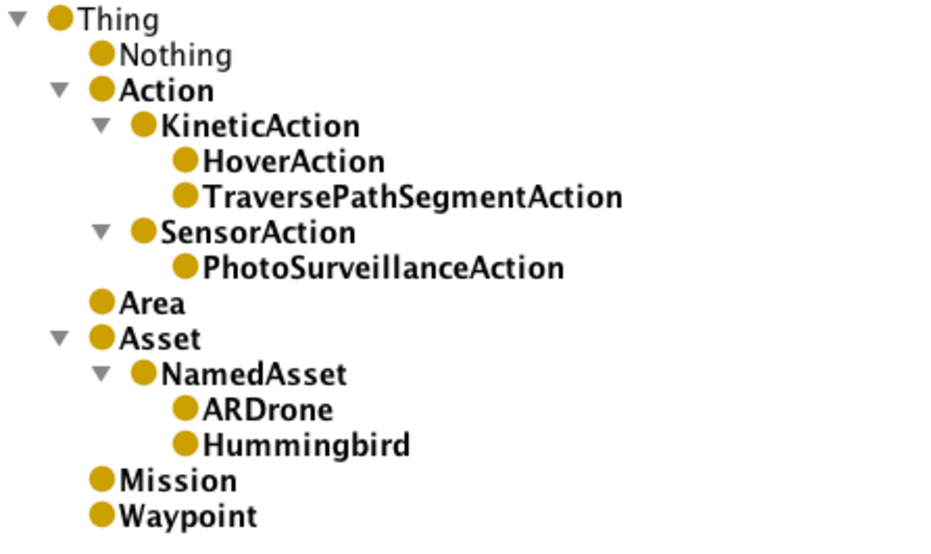
\includegraphics[scale=0.63]{img/cemo.pdf}
\caption[CEMO's class hierarchy]{CEMO's class hierarchy as presented by the Prot\'eg\'e ontology editor.}
\label{fig:complex_missions_ontology}
\end{figure}

The OWL code in Listing~\ref{lst:OWL_class_Asset} uses \emph{Manchester OWL syntax}---a human-friendly ontology representation language~\cite{Horridge_2006}---to formally defines class \texttt{Asset}, which is comprised in Mission~A\@. Lines~2--5 specify four OWL properties, which are constructs for describing relationships. In particular, an OWL property with specified \emph{domain} and \emph{range} links individuals from the domain to individuals or data values from the range. The two main OWL property types are \emph{object properties} and \emph{datatype properties}. The former describe relationships between two individuals while the latter describe relationships between individuals and data values.

\begin{lstlisting}[caption={OWL code for class \texttt{Asset}},label=lst:OWL_class_Asset]
Class: Asset
  SubClassOf: hasAction some KineticAction,
    hasCostValue some xsd:integer,
    hasEnduranceInSeconds some xsd:integer,
    hasSpeedInKilometersPerHour some xsd:integer
\end{lstlisting}

Lines~1 and~2 in Listing~\ref{lst:OWL_class_Asset} specify that every member of class \texttt{Asset} (the domain) must be associated with a member of class \texttt{KineticAction} (the range) via an instance of the object property \texttt{hasAction}. (For brevity, the reminder of this thesis will refer to \emph{property instances} simply as properties.) Members of class \texttt{Asset} are also associated with datatype properties describing asset cost, endurance and speed (lines~3--5).

Class \texttt{Asset} is extended by class \texttt{NamedAsset}, which is in turn extended by classes \texttt{ARDrone} and \texttt{Hummingbird}. The latter classes represent quadcopter UAVs manufactured by \href{http://ardrone2.parrot.com/usa/}{Parrot USA} and \href{http://www.asctec.de/}{Ascending Technologies}, respectively, that have informed our research. The OWL code in Listing~\ref{lst:OWL_class_Hummingbird} formally defines class \texttt{Hummingbird}, which is comprised in Mission~A\@.

\begin{figure}[ht]
\begin{lstlisting}[caption={OWL code for class \texttt{Hummingbird}},label=lst:OWL_class_Hummingbird]
Class: Hummingbird
  SubClassOf: NamedAsset,
    hasCostValue some xsd:integer[>= 5000],
    hasEnduranceInSeconds some xsd:integer[<= 120],
    hasSpeedInKilometersPerHour some xsd:integer[<= 50]
  DisjointWith: ARDrone
\end{lstlisting}
\end{figure}

Lines~3--5 in Listing~\ref{lst:OWL_class_Hummingbird} associate members of class \texttt{Hummingbird} with three datatype properties---\texttt{hasCostValue}, \texttt{hasEnduranceInSeconds} and \texttt{hasSpeedInKilometersPer\-Hour}. These properties are inherited from classes \texttt{NamedAsset} and, ultimately, \texttt{Asset}. Unlike class \texttt{Asset}, the ranges of the datatype properties that parameterize members of class \texttt{Hummingbird} restrict possible data values. Line~6 specifies that classes \texttt{ARDrone} and \texttt{Hummingbird} constitute \emph{disjoint} sets of individuals. Consequently, and appropriately, a member of class \texttt{ARDrone} cannot also be a member of class \texttt{Hummingbird}.

During a mission, assets execute actions that may be associated with other actions via \emph{preconditions}. An action~\emph{a} is a precondition to an action~\emph{b} if the end of~\emph{a} must precede the beginning of~\emph{b} in the sequence of actions that constitute an action workflow. Mission~A comprises three preconditions (lines~10, 18 and~22 in Listing~\ref{lst:Mission_A}), where each precondition relates actions assigned to the same asset. A fourth precondition (line~10) associates action \texttt{TPSA2} with action \texttt{TPSA3}, thereby coupling the behavior of the assets to which those actions are assigned (\texttt{H1} and~\texttt{H2}, respectively). CEMO encodes preconditions with the object property \texttt{hasPrecondition}, which is formally defined in Listing~\ref{lst:OWL_object_property_hasPrecondition}.

\begin{lstlisting}[caption={OWL code for the object property \texttt{hasPrecondition}},label=lst:OWL_object_property_hasPrecondition]
ObjectProperty: hasPrecondition
  Characteristics: Transitive
  Domain: Action
  Range: Action
  InverseOf: isPreconditionTo
\end{lstlisting}

Line~2 in Listing~\ref{lst:OWL_object_property_hasPrecondition} declares the object property \texttt{hasPrecondition} to be \emph{transitive}. Transitivity is one of several \emph{property characteristics} that can be used to qualify object properties. Given transitivity, if an action~\emph{a} is related via \texttt{hasPrecondition} to an action~\emph{b}, and~\emph{b} is related to an action~\emph{c} via the same property, then we can infer that~\emph{a} is related via \texttt{hasPrecondition} to~\emph{c}. In addition, \texttt{hasPrecondition} is inverted by the object property \texttt{isPreconditionTo} (line~5). The inverse relation between \texttt{hasPrecondition} and \texttt{isPreconditionTo} implies that if an action~\emph{a} is related via \texttt{hasPrecondition} to an action~\emph{b}, then~\emph{b} is related to~\emph{a} via \texttt{isPreconditionTo}. Figure~\ref{fig:transitive_properties} and Figure~\ref{fig:inverse_properties} illustrate transitivity and inversion, respectively.

\begin{figure}[ht]
\centering
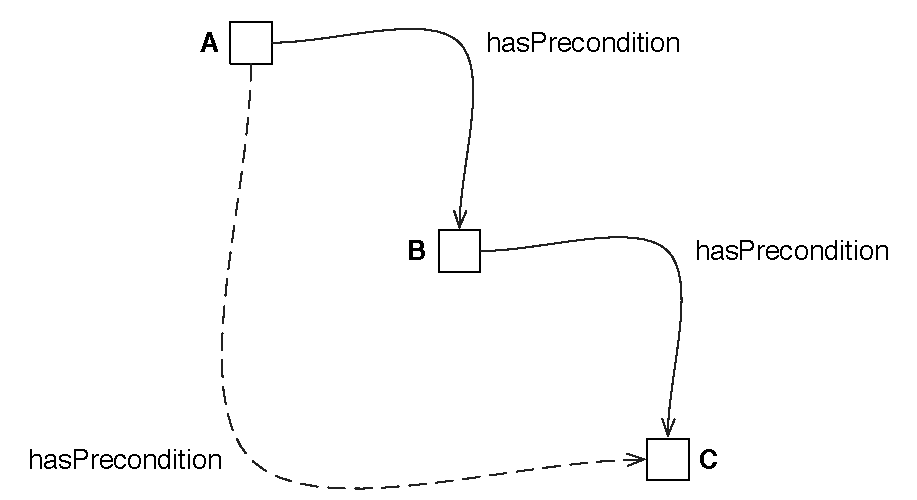
\includegraphics[scale=0.58]{img/transitive-properties.pdf}
\caption[Transitive properties]{An example of the transitive property characteristic that qualifies the object property \texttt{hasPrecondition}. The dashed line represents an inferred relationship.}
\label{fig:transitive_properties}
\end{figure}

\begin{figure}[ht]
\centering
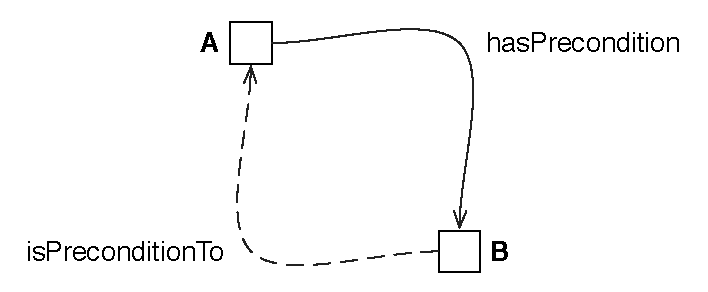
\includegraphics[scale=0.58]{img/inverse-properties.pdf}
\caption[Inverse properties]{An example of inversion with respect to the object properties \texttt{hasPrecondition} and \texttt{isPreconditionTo}. The dashed line represents an inferred relationship.}
\label{fig:inverse_properties}
\end{figure}

Because preconditions associate actions with other actions, class \texttt{Action} constitutes both the domain and range of the object property \texttt{hasPrecondition} (lines~3 and~4, respectively, in Listing~\ref{lst:OWL_object_property_hasPrecondition}). Class \texttt{Action} is extended by class \texttt{KineticAction}, whose members are associated with a data property describing action duration. Class \texttt{KineticAction} is in turn extended by classes \texttt{HoverAction} and \texttt{TraversePathSegment\-Action}. The OWL code in Listing~\ref{lst:OWL_class_TraversePathSegmentAction} formally defines class \texttt{TraversePathSegment\-Action}, which is comprised in Mission~A\@. Lines~3--4 in Listing~\ref{lst:OWL_class_TraversePathSegmentAction} specify that every member of class \texttt{TraversePathSegmentAction} must be associated via the object properties \texttt{hasStartPoint} and \texttt{hasEndpoint} with \texttt{Waypoint} individuals that designate the geographical start points and endpoints, respectively, of path segment traversal actions (hover actions are also designated geographically by waypoints).

\begin{lstlisting}[caption={OWL code for class \texttt{TraversePathSegmentAction}},label=lst:OWL_class_TraversePathSegmentAction]
Class: TraversePathSegmentAction
  SubClassOf: KineticAction,
    hasStartPoint some Waypoint,
    hasEndpoint some Waypoint
  DisjointWith: HoverAction
\end{lstlisting}

Class \texttt{Action} is also extended by class \texttt{SensorAction}, which is in turn extended by class \texttt{PhotoSurveillanceAction}. The OWL code in Listing~\ref{lst:OWL_class_PhotoSurveillanceAction} formally defines class \texttt{PhotoSurveillanceAction}, which is comprised in Mission~A\@.

\begin{lstlisting}[caption={OWL code for class \texttt{PhotoSurveillanceAction}},label=lst:OWL_class_PhotoSurveillanceAction]
Class: PhotoSurveillanceAction
  SubClassOf: SensorAction,
    hasDurationInSeconds some xsd:integer,
    hasPrecondition only Action
\end{lstlisting}

The preceding code contains the keywords \emph{some} (line~3) and \emph{only} (line~4), which represent, respectively, existential and universal restrictions in OWL\@. With regard to object properties:

\begin{itemize}

\item Existential restrictions describe classes of individuals that must participate in at least one relationship, along a specified property, with individuals that are members of a specified class~\cite{Horridge_2011}.

\item Universal restrictions describe classes of individuals that may, and can only, participate in relationships along a specified property with individuals that are members of a specified class.

\end{itemize}

\noindent Existential and universal restrictions, which can also be applied to datatype properties, are denoted in predicate logic by the existential ($\exists$) and universal ($\forall$) quantifiers, respectively.

\subsection{Modeling Tactical Missions}
\label{sec:Modeling_Tactical_Missions}

During tactical missions, assets may be required to commit threat area incursions, thereby compelling mission developers to consider the impact of asset \emph{survivability} on the probability of mission success. The United States Department of Defense (USDOD) defines survivability as ``the capability of a system \ldots\ to avoid or withstand a man-made hostile environment without suffering an abortive impairment in its ability to accomplish its designated mission.''~\cite{DoD_2001} To accommodate tactical mission requirements, we have developed a \emph{complex tactical missions ontology} (Tactical-CEMO) that extends CEMO\@.

Figure~\ref{fig:tactical_CEMO} illustrates Tactical-CEMO's multiple inheritance class hierarchy; for example, class \texttt{DirectThreatAreaHoverAction} extends classes \texttt{HoverAction} and \texttt{Threat\-AreaAction}. Classes describing tactical missions are highlighted in bold and thereby differentiate from classes encoded in CEMO\@. Used exclusively to support automated reasoning, tactical concepts are not available to mission developers via the YAML DSL\@.

\begin{figure}[ht]
\centering
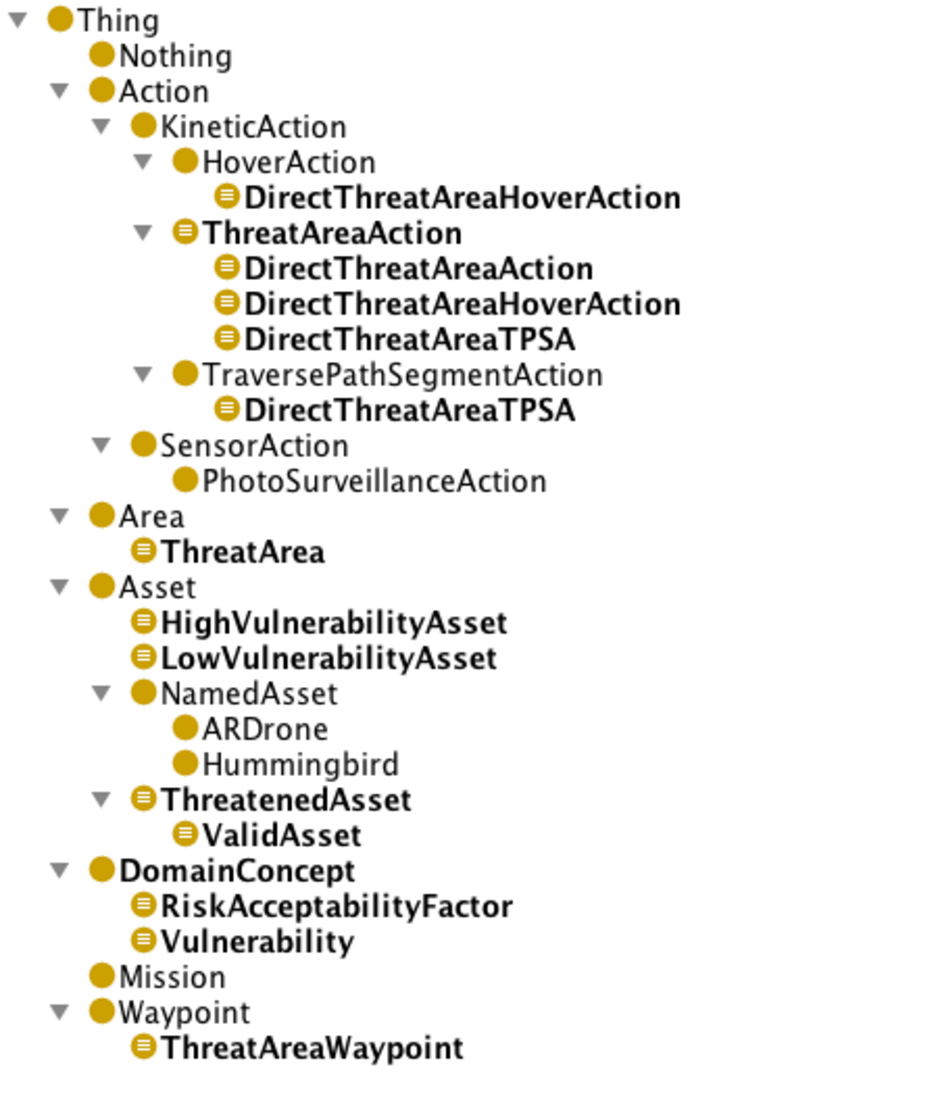
\includegraphics[scale=0.63]{img/tactical-cemo.pdf}
\caption[Tactical-CEMO's class hierarchy]{Tactical-CEMO's multiple inheritance class hierarchy as presented by the Prot\'eg\'e ontology editor.}
\label{fig:tactical_CEMO}
\end{figure}

We define class \texttt{ThreatArea} in Tactical-CEMO and specify that any waypoint related to a threat area be inferred, by Pellet or other semantic reasoners, a member of class \texttt{ThreatAreaWaypoint}. (The geographic information that relates waypoints to threat areas is determined by the CVC during preprocessing, as described in Chapter~\ref{chap:Method_Overview}.) To enable the inference of class membership, class \texttt{ThreatAreaWaypoint} must be \emph{defined} by domain experts using \emph{necessary and sufficient} conditions~\cite{Horridge_2011}. We contrast necessary and sufficient conditions with \emph{necessary} conditions, which describe all classes encoded in CEMO (as described in Section~\ref{sec:Building_an_OWL_Ontology}). These classes are known as \emph{primitive}, and cannot be used to infer class membership. For example, because class \texttt{Asset} is described using only necessary conditions, an individual that is a member of class \texttt{Asset} must satisfy those conditions. However, class membership cannot be inferred for any (random) individual that satisfies the conditions describing class \texttt{Asset}. Figure~\ref{fig:necessary_conditions} illustrates the type of reasoning supported by necessary conditions.

\begin{figure}[ht]
\centering
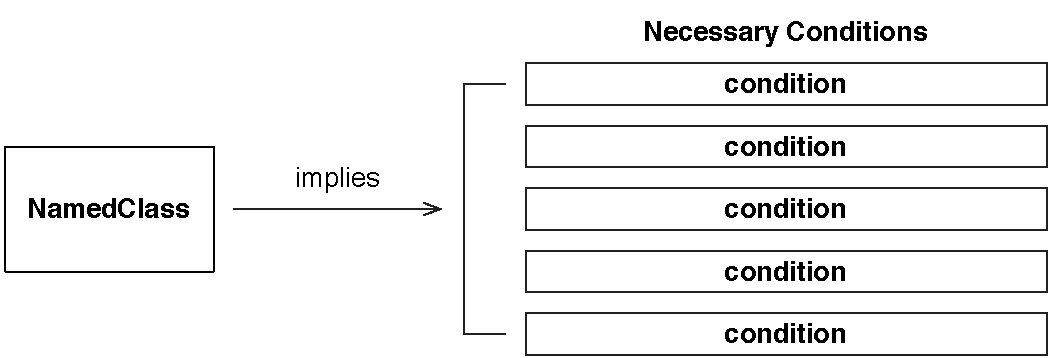
\includegraphics[scale=0.58]{img/necessary-conditions.pdf}
\caption[Primitive classes]{Necessary conditions, which describe primitive classes, cannot be used to infer class membership~\cite{Horridge_2011}. Contrast with Figure~\ref{fig:necessary_and_sufficient_conditions}, which illustrates inference underpinned by necessary and sufficient conditions.}
\label{fig:necessary_conditions}
\end{figure}

Unlike primitive classes, a \emph{defined class}, which is a class comprising necessary and sufficient conditions, can be used to infer class membership. For example, because class \texttt{ThreatAreaWaypoint} is defined using necessary and sufficient conditions, class membership can be inferred for any (random) individual that satisfies those conditions. As with primitive classes, the conditions comprised by class \texttt{ThreatAreaWaypoint} must be satisfied by its members. In other words, class \texttt{ThreatAreaWaypoint} is defined using conditions that are necessary for, and sufficient to infer, class membership. Figure~\ref{fig:necessary_and_sufficient_conditions} illustrates the type of reasoning supported by necessary and sufficient conditions. The OWL code in Listing~\ref{lst:OWL_class_ThreatAreaWaypoint} formally defines class \texttt{ThreatAreaWaypoint}, with the keyword \texttt{EquivalentTo} establishing necessary and sufficient conditions for that class.

\begin{figure}[ht]
\centering
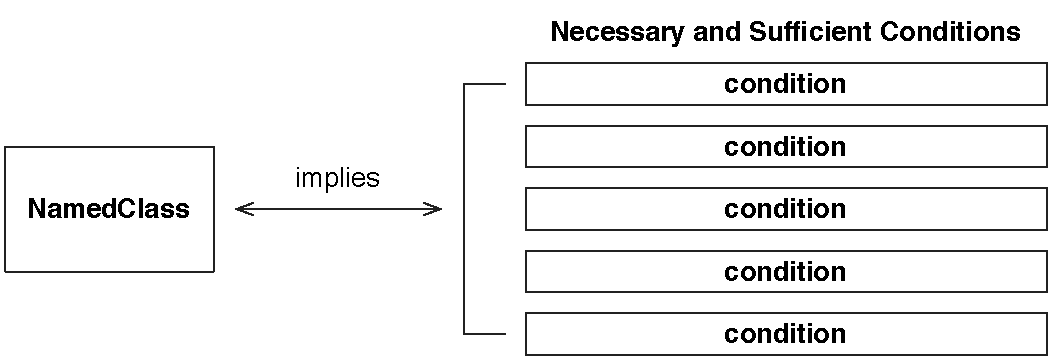
\includegraphics[scale=0.58]{img/necessary-and-sufficient-conditions.pdf}
\caption[Defined classes]{Necessary and sufficient conditions, which are comprised by defined classes, can be used to infer class membership~\cite{Horridge_2011}. Contrast with Figure~\ref{fig:necessary_conditions}, which illustrates inference underpinned by necessary conditions.}
\label{fig:necessary_and_sufficient_conditions}
\end{figure}

\begin{lstlisting}[caption={OWL code for class \texttt{ThreatAreaWaypoint}},label=lst:OWL_class_ThreatAreaWaypoint]
Class: ThreatAreaWaypoint
  EquivalentTo: Waypoint
    and (isWaypointOf some ThreatArea)
\end{lstlisting}

Since members of class \texttt{Waypoint} are associated with \texttt{HoverAction} and \texttt{Traverse\-PathSegmentAction} individuals (see Section~\ref{sec:Building_an_OWL_Ontology}), we specify that any kinetic action related to a threat area waypoint be inferred a member of class \texttt{ThreatAreaAction}. We assert the qualitative difference between \emph{threat area actions} that initiate or prolong an incursion and threat area actions that terminate an incursion, and specify that the former be inferred members of class \texttt{DirectThreatAreaAction}. We further assert the qualitative difference between \emph{direct threat area actions} (DTAAs) that execute exclusively, thereby endangering an asset seemingly without purpose, and those DTAAs that execute concurrently with one or more sensor actions. Given these assertions, we specify that assets with at least one assigned DTAA be inferred members of class \texttt{ThreatenedAsset}. We also specify that a threatened asset with assigned DTAAs be inferred a member of class \texttt{ValidAsset}, if at least one of those DTAAs executes concurrently with at least one sensor action assigned to the same asset. The OWL code in Listing~\ref{lst:OWL_class_ValidAsset} formally defines class \texttt{ValidAsset}.

\begin{lstlisting}[caption={OWL code for class \texttt{ValidAsset}},label=lst:OWL_class_ValidAsset]
Class: ValidAsset
  EquivalentTo: ThreatenedAsset
    and (hasAction some
      (SensorAction
        and (hasSibling some DirectThreatAreaAction)))
\end{lstlisting}

The preceding code contains a nested class expression that is disambiguated with parentheses. This class expression can be understood as follows: A member of class \texttt{ValidAsset} is equivalent to a threatened asset associated, via the object property \texttt{hasAction}, to a member of class \texttt{SensorAction} that is in turn associated, via the object property \texttt{hasSibling}, to a member of class \texttt{DirectThreatAreaAction}. The OWL code in Listing~\ref{lst:OWL_object_property_hasSibling} formally defines \texttt{hasSibling}.

\begin{figure}[ht]
\begin{lstlisting}[caption={OWL code for the object property \texttt{hasSibling}},label=lst:OWL_object_property_hasSibling]
ObjectProperty: hasSibling
  Characteristics: Asymmetric,
    Irreflexive
  Domain: SensorAction
  Range: KineticAction
\end{lstlisting}
\end{figure}

Lines~2 and~3 in Listing~\ref{lst:OWL_object_property_hasSibling} qualify the object property \texttt{hasSibling} with the asymmetric and irreflexive property characteristics, respectively (the transitive property characteristic was introduced in Section~\ref{sec:Building_an_OWL_Ontology}). Because \texttt{hasSibling} is asymmetric\footnote{While potentially counterintuitive, an asymmetric sibling relationship is nevertheless consistent in the context of our domain model.}, if an action~\emph{a} is related via \texttt{hasSibling} to an action~\emph{b}, then~\emph{b} cannot be related to~\emph{a} via the same property. Because \texttt{hasSibling} is irreflexive, if an action~\emph{a} is related via \texttt{hasSibling} to an action~\emph{b}, then~\emph{a} and~\emph{b} cannot be the same action. Figure~\ref{fig:asymmetric_and_irreflexive_properties} illustrates the asymmetric and irreflexive property characteristics that qualify \texttt{hasSibling}.

\begin{figure}[ht]
\centering
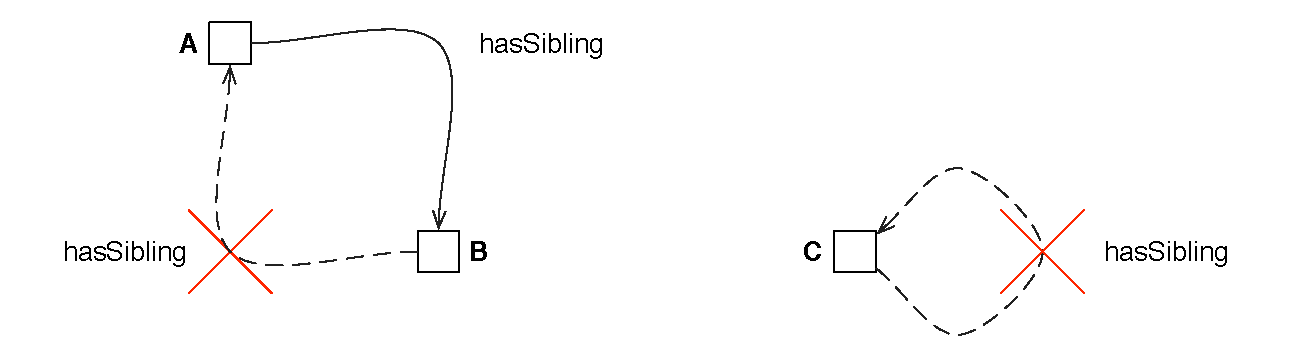
\includegraphics[scale=0.58]{img/asymmetric-irreflexive-properties.pdf}
\caption[Asymmetric and irreflexive properties]{An example of the asymmetric (left) and irreflexive (right) property characteristics that qualify the object property \texttt{hasSibling}. The dashed lines represent inferred relationships.}
\label{fig:asymmetric_and_irreflexive_properties}
\end{figure}

Classes \texttt{ThreatenedAsset} and \texttt{ValidAsset} provide an initial mission verification mechanism in the context of our method. Specifically, a mission specification is inconsistent if it contains threatened assets that are not also \emph{valid assets}. Once the validity of threatened assets has been inferred, the CVC synthesizes DTMC models that enable PRISM to compute the probability of survival for those assets. Accordingly, synthesized models encompass probabilities describing the \emph{vulnerability} of real-world assets. The USDOD defines vulnerability as ``the characteristic of a system that causes it to suffer a definite degradation \ldots\ [resulting from exposure] to a defined level of effects in a man-made hostile environment.''~\cite{DoD_2001} Vulnerability probabilities are derived from classes \texttt{HighVulnerabilityAsset} and \texttt{LowVulnerabilityAsset}, which extend class \texttt{Asset}. The OWL code in Listing~\ref{lst:OWL_class_HighVulnerabilityAsset} formally defines class \texttt{HighVulnerabilityAsset}.

\begin{figure}[ht]
\begin{lstlisting}[caption={OWL code for class \texttt{HighVulnerabilityAsset}},label=lst:OWL_class_HighVulnerabilityAsset]
Class: HighVulnerabilityAsset
  EquivalentTo: Asset
    and (hasCostValue some xsd:integer[<= 1000])
    and (hasSpeedInKilometersPerHour some xsd:integer[<= 20])
  SubClassOf:
    hasRiskAcceptabilityFactor value HighRiskAcceptabilityFactor,
    hasVulnerability value HighVulnerability
  DisjointWith: LowVulnerabilityAsset
\end{lstlisting}
\end{figure}

Similar to class \texttt{Hummingbird}, the ranges of the datatype properties that parameterize members of class \texttt{HighVulnerabilityAsset}, including \texttt{hasCostValue} and \texttt{hasSpeedIn\-KilometersPerHour} (lines~3 and~4, respectively, in Listing~\ref{lst:OWL_class_HighVulnerabilityAsset}), restrict possible datatype values. The datatype property \texttt{hasEnduranceInSeconds}, which is inherited from class \texttt{Asset} (line~2), is not calibrated in a similar manner. The decision to calibrate two of the three inherited datatype properties implies that the calibrated properties are more likely to impact asset vulnerability. We note that, unlike class \texttt{Hummingbird}, the datatype properties in Listing~\ref{lst:OWL_class_HighVulnerabilityAsset} establish necessary and sufficient conditions (lines~1--4), and thereby support the inference of membership for class \texttt{HighVulnerabilityAsset}.

Lines~6 and~7 in Listing~\ref{lst:OWL_class_HighVulnerabilityAsset} use the keyword \texttt{value} to declare \emph{hasValue} restrictions, which describe classes of individuals that must participate in at least one relationship, along a specified property, with a specific individual~\cite{Horridge_2011}. In particular, line~6 specifies that every member of class \texttt{HighVulnerabilityAsset} must be associated with the individual \texttt{HighRiskAcceptabilityFactor} via the object property \texttt{hasRiskAcceptability\-Factor} (the concept of \emph{risk acceptability} will be elaborated in Section~\ref{sec:Modeling_Risk_Acceptability}). Line~7 specifies that every member of class \texttt{HighVulnerabilityAsset} must be associated with the individual \texttt{HighVulnerability} via the object property \texttt{hasVulnerability}. The individuals \texttt{HighRiskAcceptabilityFactor} and \texttt{HighVulnerability} belong, respectively, to the \emph{enumerated classes} \texttt{RiskAcceptabilityFactor} and \texttt{Vulnerability}, which extend the generic class \texttt{DomainConcept}. An enumerated class is defined by listing precisely the individuals that are members of that class. The OWL code in Listing~\ref{lst:OWL_class_Vulnerability} formally defines class \texttt{Vulnerability}.

\begin{lstlisting}[caption={OWL code for class \texttt{Vulnerability}},label=lst:OWL_class_Vulnerability]
Class: Vulnerability
  EquivalentTo: DomainConcept
    and ({HighVulnerability, LowVulnerability})
  DisjointWith: RiskAcceptabilityFactor
\end{lstlisting}

Line~3 in Listing~\ref{lst:OWL_class_Vulnerability} specifies two individuals---\texttt{HighVulnerability} and \texttt{LowVul\-nerability}---that constitute class \texttt{Vulnerability}. The OWL code in Listing~\ref{lst:OWL_individual_HighVulnerability} formally defines the individual \texttt{HighVulnerability}, which is associated with a datatype property describing a double-precision number (line~3). The value of this number is used by the CVC to calculate probabilities that are ultimately integrated into DTMC models representing high vulnerability assets. These modules enable PRISM to compute the probability of survival for high vulnerability assets during threat area incursions. The synthesis process will be elaborated in Section~\ref{sec:Behavioral_Modeling}.

\begin{lstlisting}[caption={OWL code for the individual \texttt{HighVulnerability}},label=lst:OWL_individual_HighVulnerability]
Individual: HighVulnerability
  Types: Vulnerability
  Facts: hasDoubleValue 0.1
\end{lstlisting}

The double-precision number encapsulated by the individual \texttt{HighVulnerability} is the raison d'\^{e}tre for that individual's existence in our ontology. In other words, because datatype properties link classes to data ranges (for example, class \texttt{Hummingbird}) and individuals to data values, we were compelled to create classes of \emph{individuals} that could encapsulate risk acceptability and asset vulnerability \emph{values}. And because the number of individuals per class was finite, enumeration enabled us to explicitly declare the completeness of those classes, and thereby create a finite set of risk acceptability and asset vulnerability grades.

The preceding discussion regarding class \texttt{HighVulnerabilityAsset} applies equally to class \texttt{LowVulnerabilityAsset}, which is formally defined in Listing~\ref{lst:OWL_class_LowVulnerabilityAsset}. Datatype and object property ranges differentiate the two classes.

\begin{lstlisting}[caption={OWL code for class \texttt{LowVulnerabilityAsset}},label=lst:OWL_class_LowVulnerabilityAsset]
Class: LowVulnerabilityAsset
  EquivalentTo: Asset
    and (hasCostValue some xsd:integer[>= 3000])
    and (hasSpeedInKilometersPerHour some xsd:integer[<= 60])
  SubClassOf:
    hasRiskAcceptabilityFactor value LowRiskAcceptabilityFactor
    hasVulnerability value LowVulnerability,
  DisjointWith: HighVulnerabilityAsset
\end{lstlisting}

\subsection{Modeling Traffic Surveillance Missions}
\label{sec:Modeling_Traffic_Surveillance_Missions}

Having investigated tactical missions comprising threat area incursions, we considered a second case study involving traffic surveillance missions. In this scenario, which is conceptually similar to work presented by Heintz et al.~\cite{Heintz_2007}, deployed UAVs are required to monitor freeway traffic and notify subscribers if traffic speeds exceed minimum and nominal thresholds. To accommodate traffic surveillance mission requirements, we have developed a \emph{complex traffic surveillance missions ontology} (Traffic-CEMO) that extends CEMO\@.

Figure~\ref{fig:traffic_CEMO} illustrates Traffic-CEMO's class hierarchy. Classes describing traffic sur\-veillance missions are highlighted in bold, and thereby differentiate from classes encoded in CEMO\@. Also highlighted in bold are classes defined in CEMO that have been declared disjoint from classes defined in Traffic-CEMO\@. Used mainly to support automated reasoning, traffic surveillance concepts are generally not available to mission developers via the YAML DSL\@. Concepts available to mission developers will be highlighted in the analysis that follows.

\begin{figure}[ht]
\centering
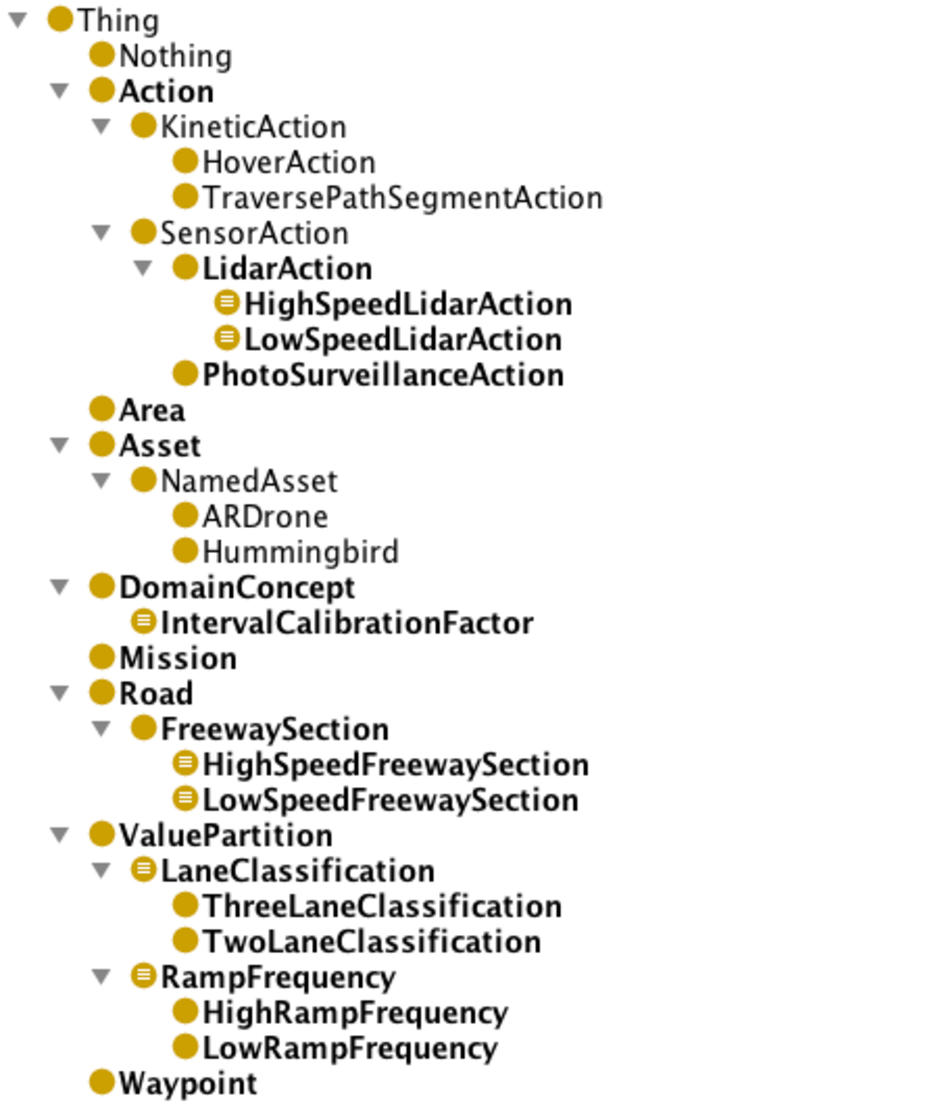
\includegraphics[scale=0.63]{img/traffic-cemo.pdf}
\caption[Traffic-CEMO's class hierarchy]{Traffic-CEMO's class hierarchy as presented by the Prot\'eg\'e ontology editor.}
\label{fig:traffic_CEMO}
\end{figure}

We define class \texttt{FreewaySection} in Traffic-CEMO and specify that two-lane freeway sections with high access ramp frequency be inferred, by Pellet or other semantic reasoners, members of \texttt{FreewaySection} subclass \texttt{LowSpeedFreewaySection}. We also specify that three-lane freeway sections with low access ramp frequency be inferred members of \texttt{FreewaySection} subclass \texttt{HighSpeedFreewaySection}. These inferred relationships formalize the correlation between off-ramp over-saturation and freeway bottlenecks that disrupt traffic discharge rates~\cite{Cassidy_2002}. The OWL code in Listing~\ref{lst:OWL_class_FreewaySection} formally defines class \texttt{FreewaySection}.

\begin{lstlisting}[caption={OWL code for class \texttt{FreewaySection}},label=lst:OWL_class_FreewaySection]
Class: FreewaySection
  SubClassOf: Road,
    approachesMinimumSpeed some xsd:double,
    exceedsMinimumSpeed some xsd:double,
    exceedsNominalSpeed some xsd:double,
    hasLaneClassification some LaneClassification,
    hasRampFrequency some RampFrequency
\end{lstlisting}

Line~3 in Listing~\ref{lst:OWL_class_FreewaySection} associates members of class \texttt{FreewaySection} with the datatype property \texttt{approachesMinimumSpeed}, which describes the potential for minimum traffic speeds to be approached during the operation of freeway sections. The datatype properties \texttt{exceedsMinimumSpeed} (line~4) and \texttt{exceedsNominalSpeed} (line~5) likewise describe the potential for minimum and nominal traffic speeds, respectively, to be exceeded during the operation of freeway sections. Lines~6 and~7 specify that every member of class \texttt{FreewaySection} must be associated, via the object properties \texttt{hasLaneClassification} and \texttt{hasRampFrequency}, with members of classes \texttt{LaneClassification} and \texttt{RampFre\-quency}, respectively. These classes extend class \texttt{ValuePartition}, which represents the \emph{value partition} design pattern~\cite{Horridge_2011}.

We use value partitions to describe the concepts of \emph{lane classification} and on/off \emph{ramp frequency}, and to restrict the range of possible values for those concepts to an exhaustive list of mutually exclusive choices. For example, class \texttt{LaneClassification} restricts the range of the object property \texttt{hasLaneClassification} to classes \texttt{TwoLaneClassifica\-tion} and \texttt{ThreeLaneClassification}. The OWL code in Listing~\ref{lst:OWL_class_LaneClassification} formally defines class \texttt{LaneClassification}.

\begin{lstlisting}[caption={OWL code for class \texttt{LaneClassification}},label=lst:OWL_class_LaneClassification]
Class: LaneClassification
  EquivalentTo: TwoLaneClassification
    or ThreeLaneClassification
  SubClassOf: ValuePartition
  DisjointWith: RampFrequency
\end{lstlisting}

Lines~1--3 in Listing~\ref{lst:OWL_class_LaneClassification} specify a \emph{covering axiom}. This type of axiom comprises a set of classes that \emph{cover} a common superclass by virtue of their union; for example, \texttt{LaneClassification} subtypes \texttt{TwoLaneClassification} and \texttt{ThreeLaneClassifi\-cation} form a union (lines~2 and~3) that covers their common superclass. We note that the union of classes \texttt{TwoLaneClassification} and \texttt{ThreeLaneClassification} establishes necessary and sufficient conditions for class \texttt{LaneClassification} (necessary and sufficient conditions were described in Section~\ref{sec:Modeling_Tactical_Missions}). The OWL code in Listing~\ref{lst:OWL_class_TwoLaneClassification} formally defines class \texttt{TwoLaneClassification}.

\begin{lstlisting}[caption={OWL code for class \texttt{TwoLaneClassification}},label=lst:OWL_class_TwoLaneClassification]
Class: TwoLaneClassification
  SubClassOf: LaneClassification
  DisjointWith: ThreeLaneClassification
\end{lstlisting}

Line~3 in Listing~\ref{lst:OWL_class_TwoLaneClassification} specifies that classes \texttt{TwoLaneClassification} and \texttt{ThreeLane\-Classification} constitute disjoint sets of individuals. Because class \texttt{LaneClassifica\-tion} is \emph{covered} by the union of its two subclasses, and because those subclasses are disjoint, a member of class \texttt{LaneClassification} must also be a member of either \texttt{TwoLaneClassification} or \texttt{ThreeLaneClassification}. As with enumeration, which was described in Section~\ref{sec:Modeling_Tactical_Missions}, value partitions enabled us to create a finite set of possible values (in this case, lane classification and ramp frequency grades). The value partitions that describe lane classification and ramp frequency are used to parameterize \texttt{FreewaySection} subtypes including classes \texttt{LowSpeedFreewaySection} and \texttt{HighSpeed\-FreewaySection}. The OWL code in Listing~\ref{lst:OWL_class_HighSpeedFreewaySection} formally defines the latter class.

\begin{figure}[ht]
\begin{lstlisting}[caption={OWL code for class \texttt{HighSpeedFreewaySection}},label=lst:OWL_class_HighSpeedFreewaySection]
Class: HighSpeedFreewaySection
  EquivalentTo: FreewaySection
    and (hasLaneClassification some ThreeLaneClassification)
    and (hasRampFrequency some LowRampFrequency)
  SubClassOf: approachesMinimumSpeed some xsd:double[>= 0.2],
    exceedsMinimumSpeed some xsd:double[>= 0.9],
    exceedsNominalSpeed some xsd:double[>= 0.5]
  DisjointWith: LowSpeedFreewaySection
\end{lstlisting}
\end{figure}

Lines~1--4 in Listing~\ref{lst:OWL_class_HighSpeedFreewaySection} use value partitions to establish necessary and sufficient conditions, and thereby support the inference of membership for class \texttt{HighSpeedFreeway\-Section}. Unlike class \texttt{FreewaySection}, the ranges of the datatype properties that parameterize members of class \texttt{HighSpeedFreewaySection} (lines~5--7) restrict possible data values. These data values specify probabilities for traffic speed fluctuations during the operation of high-speed freeway sections. Traffic speed fluctuations affect the optimal surveillance of freeway traffic by airborne \emph{light detection and ranging} (LIDAR) systems.

LIDAR is an optical remote sensing technology that can observe targets from a distance of 15 kilometers (in air) with sub-millimeter resolution~\cite{Piracha_2010}. The integration of LIDAR systems into rotary wing UAV platforms could enable, for example, a single hovering UAV with a five kilometer altitude ceiling to monitor traffic over an area spanning approximately 630 square kilometers. In the context of an urban environment, LIDAR-equipped UAVs offer a flexible and optimizable alternative to land-based cameras for the simultaneous surveillance of multiple freeway sections. The OWL code in Listing~\ref{lst:OWL_class_LidarAction} models the concept of LIDAR systems by formally defining class \texttt{LidarAction} as a sensor action subtype.

\begin{lstlisting}[caption={OWL code for class \texttt{LidarAction}},label=lst:OWL_class_LidarAction]
Class: LidarAction
  SubClassOf: SensorAction,
    hasIntervalInSeconds some xsd:integer,
    hasIntervalCalibrationFactor some IntervalCalibrationFactor,
    isConcurrentWith some HoverAction
  DisjointWith: PhotoSurveillanceAction
\end{lstlisting}

The object property \texttt{hasIntervalCalibrationFactor} (line~4 in Listing~\ref{lst:OWL_class_LidarAction}) links LIDAR actions with the individuals \texttt{HighIntervalCalibrationFactor} and \texttt{LowInter\-valCalibrationFactor}, which constitute the enumerated class \texttt{IntervalCalibration\-Factor}. Members of class \texttt{IntervalCalibrationFactor} are associated with a datatype property describing an integer. The value of this integer, which is ultimately integrated into DTMC models that simulate LIDAR actions, calibrates intervals between LIDAR readings. LIDAR intervals are specified by mission developers with a construct from our DSL; the interval type that verifies mission plans is specified by the datatype property \texttt{hasIntervalInSeconds} (line~5). Every member of class \texttt{LidarAction} is also associated, via the object property \texttt{isConcurrentWith} (line~3), with a \texttt{HoverAction} individual. This relationship is specified by mission developers via the YAML DSL\@.

Class \texttt{LidarAction} is extended by class \texttt{HighSpeedLidarAction}, which is formally defined by the OWL code in Listing~\ref{lst:OWL_class_HighSpeedLidarAction}. \texttt{LidarAction} subtype individuals are associated with members of class \texttt{HighSpeedFreewaySection} via the object property \texttt{monitors} (line~3). Given the necessary and sufficient conditions established in Listing~\ref{lst:OWL_class_HighSpeedLidarAction} (lines~1--3), LIDAR actions that monitor \emph{high-speed freeway sections} are inferred members of class \texttt{HighSpeedLidarAction}. Thus \texttt{FreewaySection} subtypes support inferences that determine the classification of \texttt{LidarAction} individuals. The object property \texttt{monitors}, which encompasses the concurrency relationship specified by mission developers, will be elaborated in Section~\ref{sec:Rule_Based_Modeling}.

\begin{lstlisting}[caption={OWL code for class \texttt{HighSpeedLidarAction}},label=lst:OWL_class_HighSpeedLidarAction]
Class: HighSpeedLidarAction
  EquivalentTo: LidarAction
    and (monitors some HighSpeedFreewaySection)
  SubClassOf: hasIntervalCalibrationFactor value HighIntervalCalibrationFactor
  DisjointWith: LowSpeedLidarAction
\end{lstlisting}

Line~4 in Listing~\ref{lst:OWL_class_HighSpeedLidarAction} links \texttt{HighSpeedLidarAction} individuals with a \emph{high interval calibration factor}, which is integrated into DTMC models representing \emph{high-speed LIDAR actions}. Thus \texttt{LidarAction} classifications support the synthesis of DTMC artifacts that model the behavior of LIDAR action individuals. The discussion regarding class \texttt{HighSpeedLidarAction} applies equally to class \texttt{LowSpeedLidarAction}, which is formally defined in Listing~\ref{lst:OWL_class_LowSpeedLidarAction}. Object property ranges differentiate the two classes.

\begin{lstlisting}[caption={OWL code for class \texttt{LowSpeedLidarAction}},label=lst:OWL_class_LowSpeedLidarAction]
Class: LowSpeedLidarAction
  EquivalentTo: LidarAction
    and (monitors some LowSpeedFreewaySection)
  SubClassOf: hasIntervalCalibrationFactor value LowIntervalCalibrationFactor
  DisjointWith: HighSpeedLidarAction
\end{lstlisting}

Appendix~\ref{chap:Ontology} presents CEMO, Tactical-CEMO and Traffic-CEMO in their entirety.

\subsection{An Overview}

Section~\ref{sec:Semantic_Modeling} exploits OWL to formalize a subset of the UAV domain. With respect to the OWL constructs presented in Section~\ref{sec:OWL_SWRL_and_Prolog}: Listing~\ref{lst:OWL_class_ThreatAreaWaypoint} uses the equivalence predicate \texttt{EquivalentTo} to establish necessary and sufficient conditions for class \texttt{ThreatArea\-Waypoint}. Listing~\ref{lst:OWL_class_Hummingbird} uses the primitive \texttt{DisjointWith} to specify that classes \texttt{ARDrone} and \texttt{Hummingbird} constitute disjoint sets. And Listing~\ref{lst:OWL_class_Vulnerability} uses enumeration to describe class \texttt{Vulnerability}. These and other OWL-based modeling methods described throughout Section~\ref{sec:Semantic_Modeling} support the expressive representation of knowledge by domain experts.

OWL also supports the efficient reasoning afforded by Pellet. Two strands of reasoning are particularly compelling because they span multiple classes and relationships. Tactical-CEMO comprises the inferred concepts \texttt{DirectThreatAreaAction} and \texttt{ValidAsset}; these concepts support the synthesis or PRISM code from templates, which will be presented in Section~\ref{sec:Modeling_Survivability} and Section~\ref{sec:Modeling_Risk_Acceptability}. Traffic-CEMO also comprises inferred concepts including \texttt{HighSpeedFreewaySection} and \texttt{HighSpeedLidarAction}, which support the synthesis of PRISM code from templates presented in Section~\ref{sec:Modeling_Traffic_Surveillance}. The OWL-based inferences described throughout Section~\ref{sec:Semantic_Modeling} enable the CVC to generate low-level system models and their desired behavioral properties from high-level system specifications encoded by model builders.

\section{Rule-Based Modeling}
\label{sec:Rule_Based_Modeling}

OWL is a powerful knowledge representation formalism, but expressive and reasoning limitations constrain its utility; for example, OWL cannot model \emph{cross-cutting actions}. We consider an action \emph{a} to be cross-cutting if~\emph{a} is a precondition to an action~\emph{b}, and~\emph{b} is assigned to an asset that is different from the asset to which~\emph{a} is assigned. By this definition, action \texttt{TPSA3} in Mission~A is a \emph{cross-cutting kinetic action}. The OWL code in Listing~\ref{lst:OWL_class_CrossCuttingKineticAction} presents an incomplete definition of class \texttt{CrossCuttingKineticAction}.

\begin{lstlisting}[caption={OWL code for class \texttt{CrossCuttingKineticAction}},label=lst:OWL_class_CrossCuttingKineticAction]
Class: CrossCuttingKineticAction
  EquivalentTo: KineticAction
    and (isActionOf some Asset)
    and (hasPrecondition some
      (Action
        and (isActionOf some Asset)))
\end{lstlisting}

The definition in Listing~\ref{lst:OWL_class_CrossCuttingKineticAction} is lacking because the asset in line~3 cannot be differentiated from the asset in line~6. The SWRL code in Listing~\ref{lst:SWRL_rule_CrossCuttingKineticAction} uses the built-in OWL property \texttt{differentFrom} to appropriately define class \texttt{CrossCuttingKineticAction} (question mark prefixes denote variables). The OWL code in line~1 provides a rudimentary definition for the \texttt{CrossCuttingKineticAction} concept, which is augmented by the rule in lines 3--12.

\begin{figure}[ht]
\begin{lstlisting}[caption={OWL+SWRL code for rule \texttt{CrossCuttingKineticAction}},label=lst:SWRL_rule_CrossCuttingKineticAction]
Class: CrossCuttingKineticAction

Rule:
    KineticAction(?a),
    KineticAction(?b),
    Asset(?x),
    Asset(?y),
    hasAction(?x, ?a),
    hasAction(?y, ?b),
    hasPrecondition(?b, ?a),
    DifferentFrom(?x, ?y)
  -> CrossCuttingKineticAction(?a)
\end{lstlisting}
\end{figure}

The SWRL rule in Listing~\ref{lst:SWRL_rule_CrossCuttingKineticAction} augments the definition of an OWL class. Listing~\ref{lst:SWRL_rule_monitors} uses a SWRL rule to augment the OWL object property \texttt{monitors}, which supports inferences described in Section~\ref{sec:Modeling_Traffic_Surveillance_Missions}. Lines~1--5 formally define \texttt{monitors} as an asymmetric and irreflexive object property with domain and range the classes \texttt{LidarAction} and \texttt{FreewaySection}, respectively (similar definitions have been introduced throughout this chapter). Line~14 specifies that a LIDAR action~\emph{?l} (defined in line~10) monitors a freeway section~\emph{?f} (defined in line~8) if the hover action~\emph{?h} (defined in line~9) that executes concurrently with~\emph{?l} (as specified in line~13) is associated with a waypoint~\emph{?w} (as specified in line~11) that also delineates~\emph{?f} (as specified in line~12).

\begin{lstlisting}[caption={OWL+SWRL code for rule \texttt{monitors}},label=lst:SWRL_rule_monitors]
ObjectProperty: monitors
  Characteristics: Asymmetric,
    Irreflexive
  Domain: LidarAction
  Range: FreewaySection

Rule:
    FreewaySection(?f),
    HoverAction(?h),
    LidarAction(?l),
    hasWaypoint(?f, ?w),
    hasWaypoint(?h, ?w),
    isConcurrentWith(?l, ?h)
  -> monitors(?l, ?f)
\end{lstlisting}

SWRL rules extend the expressive power of OWL; but like OWL, SWRL cannot reason effectively with negation. Rules that must reason with negation are therefore encoded in Prolog. Domain knowledge is negated during the ontology development process if Pellet reasoning with respect to that knowledge is deemed unattainable. The Prolog code in Listing~\ref{lst:Prolog_rule_terminal} formally defines rule \texttt{terminal}, which comprises three negated atoms (an atom is the basic building block of a Prolog rule). Rule \texttt{terminal} encapsulates both explicit and inferred ontological knowledge; explicit knowledge is encoded with the atom \texttt{has\_action} (line~2), while the three negated atoms (lines~3--5) encode knowledge inferred by Pellet.

\begin{lstlisting}[caption={Prolog code for rule \texttt{terminal}},label=lst:Prolog_rule_terminal]
terminal(X) :-
    has_action(A, X),
    not(is_precondition_to(X, _)),
    not(single_action_asset(A)),
    not(zero_action_asset(A)).
\end{lstlisting}

The transition of inferred knowledge from OWL to Prolog can be illustrated with the atom \texttt{is\_precondition\_to} (line~3 in Listing~\ref{lst:Prolog_rule_terminal}). The OWL code in Listing~\ref{lst:OWL_object_property_isPreconditionTo} formally defines the object property \texttt{isPreconditionTo}, a relationship that inverts the object property \texttt{hasPrecondition}. This inversion constitutes a Pellet inference (as described in Section~\ref{sec:Semantic_Modeling}).

\begin{lstlisting}[caption={OWL code for the object property \texttt{isPreconditionTo}},label=lst:OWL_object_property_isPreconditionTo]
ObjectProperty: isPreconditionTo
  InverseOf: hasPrecondition
  (*\ldots*)
\end{lstlisting}

Mission~A comprises several instances of the DSL construct \texttt{preconditions} (lines~10, 18 and~22 in Listing~\ref{lst:Mission_A}). The CVC transforms knowledge contained in this construct into knowledge encoded as property \texttt{hasPrecondition}. Knowledge inferred by Pellet with respect to \texttt{hasPrecondition}, via the inverted property \texttt{isPreconditionTo}, is transformed by the CVC into knowledge encoded with the atom \texttt{is\_precondition\_to}, which in turn supports SWI-Prolog inferences.

Appendix~\ref{chap:Ontology} and Appendix~\ref{chap:Prolog_Knowledge_Base} present, respectively, the SWRL and Prolog rule-bases in their entirety.

\subsection{An Overview}

Section~\ref{sec:Rule_Based_Modeling} exploits SWRL to overcome OWL limitations and encode complex relational structures. SWRL rules in Listing~\ref{lst:SWRL_rule_CrossCuttingKineticAction} and Listing~\ref{lst:SWRL_rule_monitors} augment class \texttt{CrossCutting\-KineticAction} and the object property \texttt{monitors}, respectively. The inferred concept \texttt{CrossCuttingKineticAction} supports PRISM code synthesis via a process that will be described in Chapter~\ref{chap:Cascading_Verification}. In conjunction with several inferred concepts, including \texttt{HighSpeedFreewaySection} and \texttt{HighSpeedLidarAction}, the object property \texttt{monitors} supports the synthesis of PRISM code from templates, which will be presented in Section~\ref{sec:Modeling_Traffic_Surveillance}.

Prolog is used to overcome OWL+SWRL limitations and encode knowledge that can support effective reasoning with negation. Listing~\ref{lst:Prolog_rule_terminal} and Listing~\ref{lst:OWL_object_property_isPreconditionTo} illustrate composite FOL reasoning, which is reasoning supported by multiple and integrated FOL-based systems, with the transition of inferred knowledge from OWL to Prolog. The process that leverages composite reasoning to synthesize PRISM code will be described in Chapter~\ref{chap:Cascading_Verification}.

\section{Behavioral Modeling}
\label{sec:Behavioral_Modeling}

OWL+SWRL and Prolog are appropriate formalisms for encoding semantic and rule-based knowledge. Likewise, the state-based PRISM modeling language is an appropriate formalism for encoding behavioral knowledge as DTMC models. The PRISM language can thus form the basis for reusable DTMC templates.

The code in Listing~\ref{lst:DTMC_asset_module_template} uses string interpolation, which is denoted by the code snippet \texttt{\#\{ \ldots\ \}}, to encapsulate parameters in the context of a DTMC template for asset modules. The \emph{module} is a fundamental PRISM language construct. The asset module template encodes knowledge that describes the behavior of the \texttt{Asset} concept encoded in CEMO\@.

\begin{lstlisting}[caption={DTMC template for asset modules},label=lst:DTMC_asset_module_template]
module #{asset.class}#{asset.id}
  e#{asset.id} : [0..#{asset.endurance}] init #{asset.endurance};
  (*\colorbox{yellow!25}{FOR action IN asset.kinetic\_actions DO}*)
  [#{(*{\color{blue}action.type}*)}] e#{asset.id}>0 & d#{action.id}>0
      -> (e#{asset.id}'=e#{asset.id}-1);
  (*\colorbox{yellow!25}{END}*)
  [#{(*{\color{blue}asset.last\_action.type}*)}] e#{asset.id}=0 | d#{(*{\color{purple}asset.last\_action.id}*)}=0
      -> true;
endmodule
\end{lstlisting}

A module definition contains \emph{variables} and \emph{commands}. Asset module states are stored in variable \texttt{e\#\{asset.id\}} (lines~2, 4, 5 and~7 in Listing~\ref{lst:DTMC_asset_module_template}), which represents asset endurance. Line~2 declares \texttt{e\#\{asset.id\}} to be an integer variable with range \texttt{[0..\#\{asset.endurance\}]}. The upper limit for the range is derived from \texttt{asset.en\-durance}, which also initializes \texttt{e\#\{asset.id\}} (as denoted by the keyword \texttt{init}).

Asset behavior is formalized with two or more commands, where each command assumes the form:

\begin{quote}
$[action]\:guard \rightarrow P(update_1) : update_1 + \ldots + P(update_n) : update_n;$
\end{quote}

\noindent A command becomes \emph{enabled} for execution when its \emph{guard} is satisfied by a specific model state; for example, lines~4 and~5 in Listing~\ref{lst:DTMC_asset_module_template} specify a command that becomes enabled when action duration, which is denoted by variable \texttt{d\#\{action.id\}}, \emph{and} asset endurance exceed zero. Commands encompass one or more updates, where each \emph{update} transitions a module, with a given probability, from one state to the next. A probability of one is assumed, and can therefore be omitted, for commands with single updates. Each command may be labeled with an \emph{action}, which forces two or more modules to transition states simultaneously (i.e., to synchronize).

Lines~3 and~6 in Listing~\ref{lst:DTMC_asset_module_template} use meta-code, which is highlighted with yellow background, to define a for loop. The form assumed by each for loop is

\begin{quote}
\begin{lstlisting}[frame=none,numbers=none]
(*\colorbox{yellow!25}{FOR var IN collection DO}*) body (*\colorbox{yellow!25}{END}*)
\end{lstlisting}
\end{quote}

\noindent where \texttt{var} denotes a variable and \texttt{collection} denotes a collection of objects. Each asset module command generated by the for loop in Listing~\ref{lst:DTMC_asset_module_template} represents the execution of a kinetic action. The \texttt{true} keyword in the last command (line~8) denotes the end of execution for a specific module. This type of command prevents deadlocks that are inconsequential to mission correctness from terminating the verification process with an error.

Arguments for the parameters in Listing~\ref{lst:DTMC_asset_module_template} are derived from explicit and inferred domain knowledge. Specifically, arguments for \texttt{asset.class} (line~1) and \texttt{asset.id} (lines~1, 2, 4, 5 and~7) are derived from mission plans; arguments for \texttt{asset.endurance} (line~2) are derived from explicit domain knowledge encoded in CEMO; and arguments for \texttt{action.type} (line~4), \texttt{asset.last\_action.type} (line~7) and \texttt{asset.last\_action.id} (line~7) are derived from knowledge inferred by Pellet and the Prolog compiler (via a process that will be described in Chapter~\ref{chap:Cascading_Verification}). Listing~\ref{lst:DTMC_asset_module_template} uses blue text to highlight parameters that receive as arguments domain-specific knowledge encoded by domain experts and derived from inferences. Purple text highlights parameters that receive as arguments mission-specific knowledge encoded by mission developers and also derived from inferences. This color coding scheme will be used for the remainder of Chapter~\ref{chap:Domain_Modeling}.

Mission properties are encoded in PRISM's property specification language, which subsumes several probabilistic temporal logics including PCTL, CSL and LTL\@. The code in Listing~\ref{lst:PCTL_action_duration_template} formally defines a mission property template. This generic property queries the probability that an action with identifier \texttt{action.id} will deplete its duration---as denoted by the assertion \texttt{d\#\{action.id\}=0}---and thereby complete its execution. An ellipsis indicates the potential for synthesized properties to comprise multiple assertions. Arguments for the parameter \texttt{action.id} are derived from knowledge inferred by Pellet and the Prolog compiler (via a process that will be described in Chapter~\ref{chap:Cascading_Verification}).

\begin{lstlisting}[caption={PCTL template for action duration},label=lst:PCTL_action_duration_template]
P=? [ F d#{(*{\color{purple}action.id}*)}=0 (*\ldots\hspace{1.8mm}*)]
\end{lstlisting}

\subsection{Modeling Survivability}
\label{sec:Modeling_Survivability}

Asset module commands comprise single updates that omit probabilities. The code in Listing~\ref{lst:DTMC_asset_survivability_template} formally defines a template for asset survivability modules, which contain commands with multiple updates. Survivability modules enable PRISM to calculate the probability of survival for \texttt{ValidAsset} individuals with respect to the threat area actions executed by each asset (valid assets were described in Section~\ref{sec:Modeling_Tactical_Missions}). Module states are stored in the boolean variable \texttt{a\#\{asset.id\}d} (defined in line~9 and used in lines~11--14), which represents the destruction of the asset with identifier \texttt{asset.id}. Command updates transition survivability modules from one state to the next. The probability of execution for each update is derived from the parameter \texttt{asset.vulnerability} (lines~12 and~13). Current vulnerability values are arbitrary, and should eventually be calculated from real-world data related to asset capabilities, terrain types and weather conditions.

\begin{figure}[ht]
\begin{lstlisting}[caption={DTMC template for asset survivability},label=lst:DTMC_asset_survivability_template]
(*\colorbox{yellow!25}{FOR action IN asset.threat\_area\_actions DO}*)
const int start#{(*{\color{purple}action.id}*)} = #{(*{\color{purple}action.start}*)};
const int finish#{(*{\color{purple}action.id}*)} = #{(*{\color{purple}action.finish}*)};
formula actn#{(*{\color{purple}action.id}*)}_tai = d#{(*{\color{purple}action.id}*)}>finish#{(*{\color{purple}action.id}*)} &
    d#{(*{\color{purple}action.id}*)}<=start#{(*{\color{purple}action.id}*)};
(*\colorbox{yellow!25}{END}*)

module #{(*{\color{purple}asset.class}*)}#{(*{\color{purple}asset.id}*)}_Survivability
  a#{(*{\color{purple}asset.id}*)}d : bool init false;
  (*\colorbox{yellow!25}{FOR action IN asset.threat\_area\_actions DO}*)
  [#{(*{\color{blue}action.type}*)}] !a#{(*{\color{purple}asset.id}*)}d & actn#{(*{\color{purple}action.id}*)}_tai
      -> #{1-(*{\color{purple}asset.vulnerability}*)}:(a#{(*{\color{purple}asset.id}*)}d'=false) +
         #{(*{\color{purple}asset.vulnerability}*)}:(a#{(*{\color{purple}asset.id}*)}d'=true);
  [#{(*{\color{blue}action.type}*)}] a#{(*{\color{purple}asset.id}*)}d | !actn#{(*{\color{purple}action.id}*)}_tai
      -> true;
  (*\colorbox{yellow!25}{END}*)
endmodule
\end{lstlisting}
\end{figure}

Lines~1 and~6 in Listing~\ref{lst:DTMC_asset_survivability_template} use meta-code to define a for loop that generates one \emph{formula} with identifier \texttt{actn\#\{action.id\}\_tai} (defined in line~4 and used in lines~11 and~14) per each action assigned to the asset in the loop header (the formula is a PRISM language construct used to avoid code duplication). Each formula specifies an overlap between the prosecution of a threat area incursion and the execution of a threat area action with identifier \texttt{action.id} (threat area actions were described in Section~\ref{sec:Modeling_Tactical_Missions}). This overlap is delineated by variables \texttt{start\#\{action.id\}} and \texttt{finish\#\{action.id\}} (defined in lines~2 and~3, respectively), which are assigned geographic information calculated by the CVC during preprocessing (as described in Chapter~\ref{chap:Method_Overview}).

The constructs \texttt{a\#\{asset.id\}d} and \texttt{actn\#\{action.id\}\_tai} combine to form logical expressions, including a logical conjunction and disjunction (lines~11 and~14, respectively), that constitute the guards in the asset survivability module. When these expressions are considered in union, their logical truth values, which are highlighted in Table~\ref{tab:asset_survivability_module_truth_table}, clarify asset behavior and susceptibility during threat area incursions. Specifically, a valid asset exists in one of the following disjoint states:

\begin{itemize}

\item \emph{not} destroyed and prosecuting a threat area incursion, whereby the logical conjunction is true;

\item destroyed, as a consequence of prosecuting a threat area incursion, or \emph{not} prosecuting a threat area incursion, whereby the logical disjunction is true.

\end{itemize}

\begin{table}[ht]
	\arrayrulecolor{Gray}
	\renewcommand*\arraystretch{1.3}
	\begin{tabularx}{\textwidth}{
			>{\centering\arraybackslash}X|
			>{\centering\arraybackslash}X|
			>{\centering\arraybackslash}X|
			>{\centering\arraybackslash}X
		}
		$d$ & $tai$ & $!d \wedge tai$ & $d \vee !tai$\\
		\hline
		true & true & false & \cellcolor{green!65}true\\
		\hline
		true & false & false & \cellcolor{green!65}true\\
		\hline
		false & true & \cellcolor{green!65}true & false\\
		\hline
		false & false & false & \cellcolor{green!65}true\\
	\end{tabularx}
	\caption[Asset survivability truth table]{A truth table for asset survivability guards, with variables \texttt{a\#\{asset.id\}d} and \texttt{actn\#\{action.id\}\_tai} in Listing~\ref{lst:DTMC_asset_survivability_template} represented by variables \emph{d} and \emph{tai}, respectively.}
	\label{tab:asset_survivability_module_truth_table}
\end{table}

Arguments for the parameters in Listing~\ref{lst:DTMC_asset_survivability_template} are derived from explicit and inferred domain knowledge. Specifically, arguments for \texttt{action.id} (lines~4, 5, 11 and~14), \texttt{asset.class} (line~8) and \texttt{asset.id} (lines~8, 9 and~11--14) are derived from mission plans; arguments for \texttt{asset.vulnerability} (lines~12 and~13) are derived from knowledge inferred by Pellet; arguments for \texttt{action.start} (line~2), \texttt{action.finish} (line~3) are derived from geodetic calculations and knowledge inferred by Pellet; and arguments for \texttt{action.type} (lines~11 and~14) are derived from knowledge inferred by Pellet and the Prolog compiler.

The generic property in Listing~\ref{lst:PCTL_asset_survivability_template} queries the probability that an asset with identifier \texttt{asset.id} will not be destroyed during its prosecution of threat area incursions. This mission property makes explicit the intuitive correlation between asset survivability and mission correctness.

\begin{lstlisting}[caption={PCTL template for asset survivability},label=lst:PCTL_asset_survivability_template]
P=? [ F !a#{(*{\color{purple}asset.id}*)}d (*\ldots\hspace{1.8mm}*)]
\end{lstlisting}

\subsection{Modeling Risk Acceptability}
\label{sec:Modeling_Risk_Acceptability}

We assert that, during threat area incursions, mission correctness is contingent on asset survivability \emph{and} risk acceptability. As described in Section~\ref{sec:Modeling_Tactical_Missions}, a threat area action that initiates or prolongs an incursion is inferred a member of class \texttt{DirectThreat\-AreaAction}. This inference triggers the synthesis of PRISM code that calculates a \emph{risk acceptability factor} (RAF) for the threat area incursion comprising the inferred DTAA\@. Each RAF value quantifies the risk for a specific threat area incursion, with RAF values of zero and one indicating high- and low-risk incursions, respectively. A RAF numerator represents the duration of concurrent execution between sensor actions and DTAAs during a threat area incursion; the denominator represents the aggregate duration of DTAA executions during that incursion.

The code in Listing~\ref{lst:DTMC_risk_acceptability_template} formally defines a template that enables PRISM to calculate risk acceptability with respect to the threat area incursions prosecuted by a \texttt{ValidAsset} individual. For a given asset, RAF values quantifying the incursions prosecuted by that asset are aggregated by the formula with identifier \texttt{raf\#\{asset.id\}} (line~39). Numerator and denominator for this formula are derived, respectively, from the constructs \texttt{sad\#\{asset.id\}} and \texttt{tkad\#\{asset.id\}}.

\begin{figure}[!ht]
\begin{lstlisting}[caption={DTMC template for risk acceptability},label=lst:DTMC_risk_acceptability_template]
(*\colorbox{yellow!25}{FOR action IN asset.direct\_threat\_area\_actions DO}*)
const int start#{(*{\color{purple}action.id}*)} = #{(*{\color{purple}action.start}*)};
const int finish#{(*{\color{purple}action.id}*)} = #{(*{\color{purple}action.finish}*)};
formula actn#{(*{\color{purple}action.id}*)}_tai = d#{(*{\color{purple}action.id}*)}>finish#{(*{\color{purple}action.id}*)} &
    d#{(*{\color{purple}action.id}*)}<=start#{(*{\color{purple}action.id}*)};
formula duration#{(*{\color{purple}action.id}*)} = start#{(*{\color{purple}action.id}*)} - finish#{(*{\color{purple}action.id}*)};
(*\colorbox{yellow!25}{END}*)

formula tkad#{(*{\color{purple}asset.id}*)} =
    (*\colorbox{yellow!25}{FOR action IN asset.direct\_threat\_area\_actions DO}*)
    duration#{(*{\color{purple}action.id}*)}
    + (*\colorbox{yellow!25}{IF action != asset.direct\_threat\_area\_actions.last}*)
    (*;*) (*\colorbox{yellow!25}{IF action == asset.direct\_threat\_area\_actions.last}*)
    (*\colorbox{yellow!25}{END}*)

module SensorActionCounter#{(*{\color{purple}asset.id}*)}
  sad#{(*{\color{purple}asset.id}*)} : [0..tkad#{(*{\color{purple}asset.id}*)}] init 0;
  (*\colorbox{yellow!25}{FOR action IN asset.direct\_threat\_area\_actions DO}*)
  [#{(*{\color{blue}action.type}*)}] actn#{(*{\color{purple}action.id}*)}_tai &
      (
          (*\colorbox{yellow!25}{FOR sensor\_action IN asset.sensor\_actions DO}*)
          r#{(*{\color{purple}sensor\_action.id}*)}
          | (*\colorbox{yellow!25}{IF sensor\_action != asset.sensor\_actions.last}*)
          (*\colorbox{yellow!25}{END}*)
      (*)*) &
      sad#{(*{\color{purple}asset.id}*)}<tkad#{(*{\color{purple}asset.id}*)}
      -> (sad#{(*{\color{purple}asset.id}*)}'=sad#{(*{\color{purple}asset.id}*)}+1);
  [#{(*{\color{blue}action.type}*)}] !actn#{(*{\color{purple}action.id}*)}_tai |
      !(
          (*\colorbox{yellow!25}{FOR sensor\_action IN asset.sensor\_actions DO}*)
          r#{(*{\color{purple}sensor\_action.id}*)}
          | (*\colorbox{yellow!25}{IF sensor\_action != asset.sensor\_actions.last}*)
          (*\colorbox{yellow!25}{END}*)
      (*)*)
      -> true;
  (*\colorbox{yellow!25}{END}*)
endmodule

formula raf#{(*{\color{purple}asset.id}*)} = sad#{(*{\color{purple}asset.id}*)} / tkad#{(*{\color{purple}asset.id}*)};
\end{lstlisting}
\end{figure}

Listing~\ref{lst:DTMC_risk_acceptability_template} uses a sensor action counter module (lines~16--37) to calculate the duration of concurrent execution between sensor actions and DTAAs during threat area incursions prosecuted by an asset with identifier \texttt{asset.id}. Module states are stored in variable \texttt{sad\#\{asset.id\}} (defined in line~17 and used in lines~26, 27 and~39), which is incremented by command updates. Lines~18 and~36 use meta-code to define an outer for loop that generates two commands per each DTAA assigned to the asset in the loop header. Guards for these commands encapsulate the constructs \texttt{actn\#\{action.id\}\_tai} and \texttt{r\#\{sensor\_action.id\}}.

The formula identifier \texttt{actn\#\{action.id\}\_tai} in Listing~\ref{lst:DTMC_risk_acceptability_template} (defined in line~4 and used in lines~19 and~28) represents the execution of a kinetic action during the prosecution of a threat area incursion. In the context of a sensor action counter module, the scope of formula \texttt{actn\#\{action.id\}\_tai} is limited by the outer for loop. Specifically, the outer loop generates only those identifiers associated with the execution of DTAAs (as dictated by the loop header), which constitute a subset of threat area actions assigned to the asset in the loop header.

Variable \texttt{r\#\{sensor\_action.id\}} (lines~22 and~31 in Listing~\ref{lst:DTMC_risk_acceptability_template}) couples the behavior of each sensor action counter module to the state of a sensor action module representing the execution of a sensor action with identifier \texttt{action.id}. Each counter module command is associated with a for loop (lines 21--24 and 30--33) that generates one such variable per each sensor action assigned to the asset in the loop header. Two or more variables form a logical disjunction with operands generated by an if statement (lines~23 and~32). The form assumed by each if statement is

\begin{quote}
\begin{lstlisting}[frame=none,numbers=none]
code (*\colorbox{yellow!25}{IF expression}*)
\end{lstlisting}
\end{quote}

\noindent where the \texttt{code} is executed if (and only if) the \texttt{expression} evaluates to something other than \texttt{false} or \texttt{nil}.

The constructs \texttt{actn\#\{action.id\}\_tai} and \texttt{r\#\{sensor\_action.id\}} combine to form logical expressions, including a logical conjunction and disjunction (lines~19--25 and~28--34, respectively, in Listing~\ref{lst:DTMC_risk_acceptability_template}), that constitute the guards in the sensor action counter module. When these expressions are considered in union, their logical truth values, which are highlighted in Table~\ref{tab:sensor_action_counter_module_truth_table}, clarify the conditions that increment variable \texttt{sad\#\{as\-set.id\}}. Specifically, and in accordance with its specification as described above, the RAF numerator is incremented during the prosecution of a threat area incursion, and the concurrent execution of a direct threat area action and at least one sensor action, whereby the logical conjunction is true. The execution of the update in the second command prevents inconsequential deadlocks (as described in Section~\ref{sec:Behavioral_Modeling}), whereby the logical disjunction is true. We note that the expression in line~26 prevents variable \texttt{sad\#\{asset.id\}} from exceeding its upper limit. This expression, which is required by the PRISM language, does not alter the essence of the logical truth values presented in Table~\ref{tab:sensor_action_counter_module_truth_table}.

\begin{table}[ht]
	\arrayrulecolor{Gray}
	\renewcommand*\arraystretch{1.3}
	\begin{tabularx}{\textwidth}{
			>{\centering\arraybackslash}X|
			>{\centering\arraybackslash}X|
			>{\centering\arraybackslash}X|
			>{\centering\arraybackslash}X
		}
		$tai$ & $r$ & $tai \wedge r$ & $!tai \vee !r$\\
		\hline
		true & true & \cellcolor{green!65}true & false\\
		\hline
		true & false & false & \cellcolor{green!65}true\\
		\hline
		false & true & false & \cellcolor{green!65}true\\
		\hline
		false & false & false & \cellcolor{green!65}true\\
	\end{tabularx}
	\caption[Risk acceptability truth table]{A truth table for sensor action counter guards, with variables \texttt{actn\#\{action.id\}\_tai} and \texttt{r\#\{sensor\_action.id\}} in Listing~\ref{lst:DTMC_risk_acceptability_template} represented by variables~\emph{tai} and~\emph{r}, respectively. Variable~\emph{r} may also subsume a logical disjunction comprising two or more instances of variable \texttt{r\#\{sensor\_action.id\}}.}
	\label{tab:sensor_action_counter_module_truth_table}
\end{table}

Lines~1 and~7 in Listing~\ref{lst:DTMC_risk_acceptability_template} use meta-code to define a for loop that generates one formula with identifier \texttt{duration\#\{action.id\}} (line~6) per each action assigned to the asset in the loop header. Each formula uses variables \texttt{start\#\{action.id\}} and \texttt{finish\#\{action.id\}} (lines~2 and~3, respectively) to calculate the duration of overlap between the execution of a DTAA with identifier \texttt{action.id} and the prosecution of a threat area incursion by the asset to which that DTAA is assigned. Given its function as the RAF denominator, the formula identifier \texttt{tkad\#\{asset.id\}} represents the aggregate duration of DTAA executions during incursions prosecuted by the asset with identifier \texttt{asset.id}. Formula \texttt{tkad\#\{asset.id\}} (lines~9--14) comprises a for loop that increments the RAF denominator by generating the formula identifier \texttt{duration\#\{action.id\}} as an addition operand once per each action executed by the asset in the loop header.

RAF values resulting from the execution of synthesized PRISM code are verified against a RAF threshold value, which is specified in Tactical-CEMO and integrated by the CVC into synthesized mission properties. The generic property in Listing~\ref{lst:PCTL_risk_acceptability_template} queries the probability that the specified RAF value exceeds 60 percent. This threshold is encapsulated by the individual \texttt{LowRiskAcceptabilityFactor}, which belongs to the enumerated class \texttt{RiskAcceptabilityFactor} described in Section~\ref{sec:Modeling_Tactical_Missions}. Current threshold values are arbitrary, and should eventually be calculated from real-world data related to operational assessments.

\begin{figure}[ht]
\begin{lstlisting}[caption={PCTL template for risk acceptability},label=lst:PCTL_risk_acceptability_template]
P=? [ F raf#{(*{\color{purple}asset.id}*)}>0.6 (*\ldots\hspace{1.8mm}*)]
\end{lstlisting}
\end{figure}

Arguments for the parameters in Listing~\ref{lst:DTMC_risk_acceptability_template} are derived from explicit and inferred domain knowledge. Specifically, arguments for \texttt{action.id} (lines~2--6, 11, 19 and~28), \texttt{asset.id} (lines~9, 16, 17, 26, 27 and~39) and \texttt{sensor\_action.id} (lines~22 and~31) are derived from mission plans; arguments for \texttt{action.start} (line~2), \texttt{action.finish} (line~3) are derived from geodetic calculations and knowledge inferred by Pellet; and arguments for \texttt{action.type} (lines~19 and~28) are derived from knowledge inferred by Pellet and the Prolog compiler.

\subsection{Modeling Traffic Surveillance}
\label{sec:Modeling_Traffic_Surveillance}

Section~\ref{sec:Modeling_Traffic_Surveillance_Missions} describes a case study whereby LIDAR-equipped UAVs monitor freeway traffic and notify subscribers if traffic speed exceeds specified thresholds. Traffic speed fluctuations in turn affect the optimal surveillance of freeway traffic by monitoring assets. Specifically, when traffic speed descends below the nominal speed threshold, and thereby approaches the minimum speed threshold, of a freeway section~\emph{fs}, the sample rate of the LIDAR action~\emph{la} monitoring~\emph{fs} is increased by a factor equal to the calibration value associated with the conjunction of~\emph{la} and~\emph{fs}. Increased LIDAR sample rates afford fine-grained traffic control (via some process that is outside the scope of our method), which is assumed to be an appropriate mechanism for mitigating traffic congestion and bottlenecks.

Conversely, when traffic speed ascends above the nominal speed threshold, and is thereby distanced from the minimum speed threshold, of freeway section~\emph{fs}, the sample rate of~\emph{la} is decreased by a factor equal to the calibration value associated with the conjunction of~\emph{la} and~\emph{fs}. Decreased LIDAR sample rates afford coarse-grained traffic control, which is assumed to be acceptable during periods of decreased freeway traffic. LIDAR calibration can thus optimize the surveillance of multiple freeway sections by a single UAV\@.

In this context, we consider the following mission scenario:

\begin{enumerate}

\item Traffic speed exceeds the nominal speed threshold of freeway section~\emph{fs}.

\item The system optimizes its surveillance operation by decreasing the sample rate of~\emph{la} with respect to~\emph{fs}.

\item Subsequently, and during what is now a prolonged~\emph{la} interval, traffic speed descends rapidly below the minimum speed threshold of~\emph{fs}.

\end{enumerate}

\noindent Steps~2 and~3 in this scenario highlight potentially conflicting mission requirements. The system must achieve optimized performance with limited resources. Concurrently, to manage freeway traffic in real-time, the system must disseminate timely (and potentially low-latency) information from ISR assets to human and software traffic control agents. The latter requirement could presumably be compromised if~\emph{la} remains inactive for a considerable period of time following the occurrence of step~3.

Listing~\ref{lst:DTMC_traffic_surveillance_template} formally defines a template that enables PRISM to quantify probabilistically the correlation between decreased LIDAR sample rates and increased latency in the dissemination of information related to traffic speed fluctuations. Lines~27 and~41 use meta-code to define a for loop that generates one freeway section module with identifier \texttt{FreewaySection\#\{section.id\}} (line~28) per each freeway section assigned to the asset in the loop header (freeway sections are assigned to specific assets via inferences supported by the object property \texttt{monitors}, which was described in Section~\ref{sec:Modeling_Traffic_Surveillance_Missions} and Section~\ref{sec:Rule_Based_Modeling}). Freeway section modules enable PRISM to simulate traffic speed fluctuations for high- and low-speed freeways. Module states representing disjoint traffic speed intervals are stored in variable \texttt{spd\#\{section.id\}} (defined in line~29 and used in lines~14, 19 and~30--39). Three intervals describe minimum (denoted by the integer~0), nominal (1) and greater than nominal (2) traffic speeds.

\begin{figure}[!ht]
\begin{lstlisting}[caption={DTMC template for traffic surveillance},label=lst:DTMC_traffic_surveillance_template]
(*\colorbox{yellow!25}{FOR action IN asset.lidar\_actions DO}*)
const int i#{action.id} = #{action.interval};
const int icf#{action.id} = #{(*{\color{blue}action.interval\_calibration\_factor}*)};
formula ci#{action.id} = nse#{action.id}
    ? i#{action.id} * icf#{action.id}
    : i#{action.id};

module LidarAction#{action.id}
  r#{action.id} : [0..#{action.concurrent_action.duration}] init 0;
  nse#{action.id} : bool init false;
  [#{(*{\color{blue}action.concurrent\_action.type}*)}]
      mod(d#{action.concurrent_action.id}, ci#{action.id})=0 &
      r#{action.id}<#{action.concurrent_action.duration} &
      spd#{(*{\color{blue}action.section.id}*)}=2
      -> (r#{action.id}'=r#{action.id}+1) & (nse#{action.id}'=true);
  [#{(*{\color{blue}action.concurrent\_action.type}*)}]
      mod(d#{action.concurrent_action.id}, ci#{action.id})=0 &
      r#{action.id}<#{action.concurrent_action.duration} &
     !spd#{(*{\color{blue}action.section.id}*)}=2
      -> (r#{action.id}'=r#{action.id}+1) & (nse#{action.id}'=false);
  [#{(*{\color{blue}action.concurrent\_action.type}*)}]
     !mod(d#{action.concurrent_action.id}, ci#{action.id})=0
      -> true;
endmodule
(*\colorbox{yellow!25}{END}*)

(*\colorbox{yellow!25}{FOR section IN asset.freeway\_sections DO}*)
module FreewaySection#{section.id}
  spd#{section.id} : [0..2] init 1;
  [#{(*{\color{blue}section.action.concurrent\_action.type}*)}] spd#{section.id}=0
      -> #{1-(*{\color{blue}section.exceeds\_minimum\_speed}*)}:(spd#{section.id}'=0) +
         #{(*{\color{blue}section.exceeds\_minimum\_speed}*)}:(spd#{section.id}'=1);
  [#{(*{\color{blue}section.action.concurrent\_action.type}*)}] spd#{section.id}=1
      -> #{(*{\color{blue}section.approaches\_minimum\_speed}*)}:(spd#{section.id}'=0) +
         #{1-((*{\color{blue}section.exceeds\_nominal\_speed}*) + (*{\color{blue}section.approaches\_minimum\_speed}*))}:(spd#{section.id}'=1) +
         #{(*{\color{blue}section.exceeds\_nominal\_speed}*)}:(spd#{section.id}'=2);
  [#{(*{\color{blue}section.action.concurrent\_action.type}*)}] spd#{section.id}=2
      -> #{1-(*{\color{blue}section.exceeds\_nominal\_speed}*)}:(spd#{section.id}'=1) +
         #{(*{\color{blue}section.exceeds\_nominal\_speed}*)}:(spd#{section.id}'=2);
endmodule
(*\colorbox{yellow!25}{END}*)
\end{lstlisting}
\end{figure}

Command updates transition freeway section modules from one state to the next as follows: The first command derives the probability of transitioning from minimum to nominal speed via the parameter \texttt{section.exceeds\_minimum\_speed} (line~32 in Listing~\ref{lst:DTMC_traffic_surveillance_template}). The negation of this parameter determines the probability of maintaining minimum speed (line~31).

The second command derives the probability of transitioning from nominal to minimum speed via the parameter \texttt{section.approaches\_minimum\_speed} (line~34 in Listing~\ref{lst:DTMC_traffic_surveillance_template}); the probability of transitioning from nominal to greater than nominal speed is derived via the parameter \texttt{section.exceeds\_nominal\_speed} (line~36). The sum of these parameters is negated to determine the probability of maintaining nominal speed (line~35).

The third command derives the probability of maintaining greater than nominal speed via the parameter \texttt{section.exceeds\_nominal\_speed} (line~39 in Listing~\ref{lst:DTMC_traffic_surveillance_template}). The negation of this parameter determines the probability of transitioning from greater than nominal to nominal speed (line~38). Arguments for \texttt{section.approaches\_minimum\_speed}, \texttt{section.exceeds\_minimum\_speed} and \texttt{section.exceeds\_nominal\_speed} are derived via inferences from explicit domain knowledge encoded in CEMO (as described in Section~\ref{sec:Modeling_Traffic_Surveillance_Missions}). Current probabilities are arbitrary, and should eventually be calculated from real-world data related to freeway surveillance operations.

Lines~1 and~25 in Listing~\ref{lst:DTMC_traffic_surveillance_template} use meta-code to define a for loop that generates one LIDAR action module with identifier \texttt{LidarAction\#\{action.id\}} (line~8) per each LIDAR action assigned to the asset in the loop header. Module states are stored in variables \texttt{r\#\{action.id\}} (defined in line~9 and used in lines~13, 15, 18 and~20) and \texttt{nse\#\{action.id\}} (defined in line~10 and used in lines~4, 15 and~20). The former variable represents LIDAR readings; for any given LIDAR action, the latter variable represents a transition to greater than nominal traffic speed for the freeway section monitored by that action.

Line~9 in Listing~\ref{lst:DTMC_traffic_surveillance_template} declares \texttt{r\#\{action.id\}} to be an integer variable with range \texttt{[0..\#\{action.concurrent\_action.duration\}]}. This variable is incremented by updates in two commands (lines~11--20), which represent the execution of LIDAR actions; a third command uses the \texttt{true} keyword (line~23) to represent execution intervals. Each command is enabled, either primarily or exclusively, by a modulo operation (lines~12, 17 and~22) between the constructs \texttt{d\#\{action.concurrent\_action.id\}} and \texttt{ci\#\{action.id\}}.

Variable \texttt{d\#\{action.concurrent\_action.id\}} (lines~12, 17 and~22 in Listing~\ref{lst:DTMC_traffic_surveillance_template}) represents the duration of the hover action that executes concurrently with the LIDAR action represented by variable \texttt{action}; formula \texttt{ci\#\{action.id\}} (lines~4--6) calibrates the sample rate of this LIDAR action with variables \texttt{i\#\{action.id\}} (defined in line~2 and used in lines~5 and~6) and \texttt{icf\#\{action.id\}} (defined in line~3 and used in line~5). Specifically, the LIDAR action interval \texttt{i\#\{action.id\}} is calibrated by the interval calibration factor \texttt{icf\#\{action.id\}} (as described in Section~\ref{sec:Modeling_Traffic_Surveillance_Missions}) when \texttt{nse\#\{action.id\}==true}, i.e., when traffic speed exceeds the nominal speed threshold of the freeway section monitored by the LIDAR action with identifier \texttt{action.id}. Variable \texttt{nse\#\{action.id\}} is updated, by the same commands that update \texttt{r\#\{action.id\}}, when variable \texttt{spd\#\{section.id\}} transitions between values representing minimum/nominal and greater than nominal traffic speeds. The commands that update variables \texttt{r\#\{ac\-tion.id\}} and \texttt{nse\#\{action.id\}} comprise expressions to prevent \texttt{r\#\{action.id\}} from exceeding its upper limit (lines~13 and~18). These expressions, which are required by the PRISM language, do not alter the essence of the functionality afforded by LIDAR action modules.

Listing~\ref{lst:DTMC_traffic_surveillance_template} labels all commands with actions that synchronize the execution of PRISM modules. Synchronization has been used throughout Section~\ref{sec:Behavioral_Modeling} to accurately model tightly-coupled units of behavior including LIDAR actions and the freeway sections monitored by those actions. The relationship between modeling accuracy and synchronization will be elaborated in Chapter~\ref{chap:Cascading_Verification}.

Arguments for the parameters in Listing~\ref{lst:DTMC_traffic_surveillance_template} are derived from explicit and inferred domain knowledge. Specifically, arguments for \texttt{action.id} (lines~2--6, 8--10, 12, 13, 15, 17, 18, 20 and~22), \texttt{action.interval} (line~2), \texttt{action.concurrent\_action.duration} (lines~9, 13 and~18) and \texttt{action.concurrent\_action.id} (lines~12, 17 and~22) are derived from mission plans; arguments for \texttt{action.interval\_calibration\_factor} (line~3), \texttt{ac\-tion.section.id} (lines~14 and~19), \texttt{section.exceeds\_minimum\_speed} (lines~31 and~32), \texttt{section.approaches\_minimum\_speed} (lines~34 and~35) and \texttt{section.exceeds\_nomi\-nal\_speed} (lines~35, 36, 38 and~39) are derived from knowledge inferred by Pellet; arguments for \texttt{action.concurrent\_action.type} (lines~11, 16 and~21) and \texttt{section.ac\-tion.concurrent\_action.type} (lines~30, 33 and~37) are derived from knowledge inferred by Pellet and the Prolog compiler; and arguments for \texttt{section.id} (lines~28--39) are derived from explicit domain knowledge encoded in Traffic-CEMO\@.

Lines~1 and~5 in Listing~\ref{lst:PCTL_traffic_surveillance_template} use meta-code to define a for loop that generates one property per each LIDAR action assigned to the asset in the loop header. Each property comprises a conjunction of three assertions, which verify the mission scenario described in the beginning of this section and reproduced below.

\begin{enumerate}

\item According to the assertion in line~2, traffic speed exceeds the nominal speed threshold of a freeway section that is monitored by the LIDAR action with identifier \texttt{action.id}.

\item Given the assertion in line~2, the system optimizes its surveillance operation by decreasing the sample rate of the monitoring LIDAR action.

\item The assertion in line~3 denotes that traffic speed descends below the minimum speed threshold of the freeway section with identifier \texttt{action.section.id}; in conjunction, the assertion in line~4 denotes that traffic speed decent occurs while the monitoring LIDAR action is in the process of what is now a prolonged (as a consequence of step~2) interval.

\end{enumerate}

\begin{lstlisting}[caption={PCTL template for traffic surveillance},label=lst:PCTL_traffic_surveillance_template]
(*\colorbox{yellow!25}{FOR action IN asset.lidar\_actions DO}*)
P=? [ F nse#{action.id} &
        spd#{(*{\color{blue}action.section.id}*)}=0 &
       !mod(d#{action.concurrent_action.id}, ci#{action.id})=0(*\hspace{1.8mm}*)]
(*\colorbox{yellow!25}{END}*)
\end{lstlisting}

We note that the generic property encoded in Listing~\ref{lst:PCTL_traffic_surveillance_template} is the raison d'\^{e}tre for the existence of variable \texttt{nse\#\{action.id\}}. The DTMC template in Listing~\ref{lst:DTMC_traffic_surveillance_template} declares and updates several occurrences of \texttt{nse\#\{action.id\}}, which is used by the formula \texttt{ci\#\{action.id\}}. In this context, \texttt{nse\#\{action.id\}} duplicates data stored in, and could therefore be replaced by, variable \texttt{spd\#\{section.id\}}. But the PCTL template uses \texttt{nse\#\{action.id\}} (as an assertion) to verify the sequence of steps that constitute the traffic surveillance mission scenario. In particular, \texttt{nse\#\{action.id\}} is used in conjunction with the assertion \texttt{spd\#\{action.section.id\}=0} to verify that traffic speed exceeds the nominal speed threshold, and \emph{subsequently} descends below the minimum speed threshold, of a specific freeway section.

The artifacts presented in this section enable PRISM to verify the occurrence of what is presumably a compromising scenario for traffic surveillance missions. This scenario is underpinned by three assertions, which signify failure of a LIDAR-based surveillance system to disseminate traffic speed data in a timely manner. Two assertions (lines~3 and~4 in Listing~\ref{lst:PCTL_traffic_surveillance_template}) verify the occurrence of the scenario unless traffic speed decent and reaction to that descent by the monitoring LIDAR action occur simultaneously (i.e., in the same time-step). Future work could extend PRISM artifacts to verify the occurrence of the scenario unless reaction to traffic speed decent by the monitoring LIDAR action occurs within a specified timeframe, whereby, for example, reaction time after calibration does not exceed reaction time before calibration. This type of analysis will probably afford more valuable and pertinent insight into the impact of the compromising scenario on mission correctness. Future work could also develop models and properties to analyze the surveillance of multiple freeway sections by a single LIDAR action. Additional limitations and potential for future work will be considered in Chapter~\ref{chap:Conclusions_and_Future_Work}.

These considerations do not diminish the utility of the current model: PRISM uses artifacts that encode Mission~5b, one of the~58 mission plans supporting the evaluation in Chapter~\ref{chap:Evaluation}, to verify the occurrence of the scenario described above with probabilities of approximately 0.651 and 0.625 for high- and low-speed freeway sections, respectively. PRISM verifies the occurrence of a similar scenario, but one that does \emph{not} calibrate LIDAR actions, with probabilities of approximately 0.468 and 0.525 for high- and low-speed freeway sections, respectively. These results quantify the intuitive correlation between decreased LIDAR sample rates and increased latency in the dissemination of information related to traffic speed fluctuations. Latency resulting from calibration is on average 1.391 and 1.19 times greater than latency sans calibration for high- and low-speed freeway sections, respectively. Assessing the impact of increased latency on traffic control and traffic discharge rates is beyond the scope of this thesis.

Appendix~\ref{chap:PRISM_Templates} presents DTMC and PCTL templates in their entirety. Output from these templates, and additional probabilistic results, will be presented in Chapter~\ref{chap:Cascading_Verification}.

\subsection{An Overview}

Section~\ref{sec:Behavioral_Modeling} exploits PRISM's model and property specification languages to formally define DTMC and PCTL templates, respectively. PRISM templates support the synthesis of system models and the behavioral properties that need to be verified with respect to those models. The synthesis process receives data from a variety of heterogeneous sources including system specifications; explicit knowledge formalized in CEMO, and Tactical- and Traffic-CEMO; inferred knowledge derived exclusively from Pellet-based reasoning; and inferred knowledge derived from composite, Pellet- and Prolog-based, reasoning. Inferences are generated from domain- and mission-specific knowledge encoded by domain experts and mission developers, respectively.

Templates presented in Section~\ref{sec:Modeling_Survivability} enable PRISM to calculate the probability of survival for valid assets. Each valid asset executes one or more direct threat area actions during the prosecution of a threat area incursion. PRISM quantifies the inherent risk for each incursion with synthesized code from the templates presented in Section~\ref{sec:Modeling_Risk_Acceptability}. The synthesis of PRISM code from survivability and risk acceptability templates is supported, in part, by the inferred concepts \texttt{DirectThreatAreaAction} and \texttt{ValidAsset}, which are formalized in Tactical-CEMO\@.

Section~\ref{sec:Modeling_Traffic_Surveillance} presents templates that enable PRISM to quantify the dynamic relationship between LIDAR actions and the freeway sections monitored by those actions. The synthesis of PRISM code from traffic surveillance templates is supported, in part, by the inferred concepts \texttt{HighSpeedFreewaySection} and \texttt{HighSpeedLidarAction}, and the inferred object property \texttt{monitors}, which are formalized in Traffic-CEMO\@.

\section{Related Work}
\label{sec:Domain_Modeling_Related_Work}

The work presented thus far has been broadly concerned with the (loose) integration of OWL+SWRL and Prolog, and with multi-dimensional, i.e., semantic, rule-based and behavioral, modeling in the context of the UAV domain. The following sections describe related work for each activity.

\subsection{Integrating OWL and Prolog}

\c{S}ensoy et al.\ integrate DL- and LP-based reasoning by embedding ontological terms---including classes, properties and individuals---in logic programs; the interpretation of ontological axioms is delegated to a semantic reasoner during the execution of those programs~\cite{Sensoy_2011}. The resulting method, which retains the expressivity of both OWL and Prolog, has been used to support resource determination and allocation by intelligent agents~\cite{Sensoy_2012}. With respect to the UAV domain, the method has been used by de Mel et al.\ to develop a solution for sensor assignment during ISTAR missions~\cite{De_Mel_2013}.

Matzner and Hitzler achieve DL-LP integration with a Prolog extension based on any-world semantics that uses special atoms to query the DL-reasoner KAON2~\cite{Matzner_2007}. Programs written in this language are transformed to standard LP programs encoded in SWI-Prolog. Papadakis et al.\ transform OWL ontologies to SWI-Prolog code via subject-predicate-object triplets~\cite{Papadakis_2011}. Samuel et al.\ achieve a similar transformation---from OWL+SWRL to Prolog---via a combination of XSLT templates and Prolog rules, which are used to enforce OWL primitives~\cite{Samuel_2008}. With their work, Samuel et al.\ claim to address OWL-LP integration issues related to, for example, class disjointness and enumeration that are considered unsolvable by Volz et al~\cite{Volz_2003}. Obrst et al.\ use the resulting method to rapidly integrate \emph{command-and-control} (C2) systems with new sources of information~\cite{Obrst_2010}.

The algorithm presented by Zombori transforms a TBox encoded with the description logic $\mathcal{SHIQ}$ to a set of first-order clauses~\cite{Zombori_2008}. Luk\'{a}csy and Szeredi incorporate this algorithm into a reasoning system named DLog, which generates Prolog programs from first-order clauses~\cite{Lukacsy_2009a}. Extensions to DLog introduce optimization techniques including partial evaluation, which avoids the execution of unary predicates with uninstantiated arguments~\cite{Lukacsy_2008}; and parallel query execution~\cite{Lukacsy_2009b}.

Almendros-Jim\'{e}nez uses Prolog as a query language for OWL~\cite{Almendros_Jimenez_2011}. Each query, which is encoded as a Prolog goal, retrieves data and meta-data from a given ontology. Conversely, Elenius uses OWL+SWRL to generate queries for XSB Prolog, an open source implementation of the Prolog language~\cite{Elenius_2012}. Both approaches are limited to a subset of OWL\@.

As mentioned in Chapter~\ref{chap:Background}, this thesis does not claim a contribution to the state of the art in OWL-LP integration. We have nevertheless developed a composite inference mechanism that is distinct from related work. This mechanism is perhaps most compatible with the method presented by \c{S}ensoy et al. Similarities include the delineation of OWL and Prolog with respect to the syntactic features and reasoning capabilities afforded by each language. But our mechanism executes semantic and Prolog-based reasoning in strict succession while \c{S}ensoy et al.\ interlace semantic reasoning with the execution of Prolog programs. Related work that either transforms ontological axioms to Prolog code~\cite{Papadakis_2011,Samuel_2008,Lukacsy_2009a}, or uses ontological axioms to query Prolog (or vice versa)~\cite{Almendros_Jimenez_2011,Elenius_2012}, is even further removed from our implementation of composite reasoning.

\subsection{Modeling the UAV Domain}

The technologies presented throughout this chapter have been used in related work to model aspects of the UAV domain. De Mel et al.\ and Preece et al.\ describe ontologies for UAV-based ISTAR missions~\cite{De_Mel_2013,Preece_2008}. Schumann et al.\ use OWL to formalize civilian-oriented UAV missions comprising a combination of three possible goals: loitering, path traversal and search~\cite{Ferraro_2012}. Valente et al.\ exploit OpenCyc, a general purpose knowledge base, to create ontologies for military UAV missions~\cite{Valente_2005}. Schlenoff and Messina have developed a \emph{robot ontology} that supports urban \emph{search and rescue} (S\&R) efforts by the U.S. Department of Homeland Security (DHS). The ontology encodes concepts that model \emph{aerial robots} including \emph{high altitude loiter robots}, \emph{ledge access robots} and \emph{rooftop payload drop robots}~\cite{Schlenoff_2005}.

In a more general context of robotics, Amigoni and Arrigoni Neri use an ontology to achieve resource determination and allocation with respect to a multi-robot system and its assigned tasks~\cite{Amigoni_2005}. Chella et al.\ describe a spatial ontology that models robotic knowledge regarding indoor office environments~\cite{Chella_2002}. Ontologies are exploited by Schlenoff et al.\ to enhance the navigation capabilities of autonomous vehicles~\cite{Schlenoff_2003}. Gavshin and Shumik transform ontological knowledge into executable robot control code~\cite{Gavshin_2011}.

Bohn models search and destroy missions as a pursuer-evader game, where pursuing UAVs attempt to locate evasive targets~\cite{Bohn_2007}. Model checking is subsequently used to generate strategies that are favorable for pursuers, when those strategies exist. Webster et al.\ apply model checking to the verification of high-level decision making by autonomous UASs in civilian airspace~\cite{Webster_2011}. Basic and more advanced UAS control systems are modeled with PROMELA and the autonomous agent language Gwendolen, respectively. The models are verified by Spin and the agent model checker AJPF against air traffic regulations issued by the UK Civil Aviation Authority.

Jeyaraman et al.\ use Kripke semantics to model cooperative search underpinned by Dubins paths\footnote{A Dubins path is the shortest path with bounded curvature between two points in the Euclidean plane.}~\cite{Jeyaraman_2005}. Kripke semantics are also used by Sirigineedi et al.\ to model UAV behavior during the execution of a distributed control strategy, where assets cooperate to monitor a road network~\cite{Sirigineedi_2011}. The latter model is verified by the model checker SMV against mission properties expressed in CTL\@.

Our modeling effort overlaps, to some extent, with related work presented in this section. CEMO formally defines hover and path segment traversal actions, which are similar (if not equivalent) to the loitering and path traversal goals described by Schumann et al. Tactical- and Traffic-CEMO encode military- and civilian-oriented mission concepts, respectively, and thereby resemble ontologies that formalize ISTAR and S\&R missions~\cite{De_Mel_2013,Preece_2008,Schlenoff_2005}. But unlike related work aimed at enhancing UAV capabilities~\cite{Schlenoff_2003,Bohn_2007}, we use semantic and behavioral models to verify the correctness of UAV mission plans. And unlike Gavshin and Shumik, we transform ontological (and other) knowledge into PRISM code.

Ultimately, the divergence between our work and that of others is most compelling at the intersection of semantic and behavioral modeling. This divergence will be highlighted in Chapter~\ref{chap:Cascading_Verification}.

\section{Summary}
\label{sec:Domain_Modeling_Summary}

This chapter is necessarily extensive. We exploit five formalisms---including knowledge representation languages (OWL and SWRL), a logic programming language (Prolog), a behavioral modeling language (PRISM DTMC), and a property specification language (PRISM PCTL)---to model a non-trivial application domain; in doing so, a subset of that domain is encoded precisely and from multiple perspectives. Syntactic and semantic features of each formalism, and the inherent limitations of OWL+SWRL, are described in the context of two case studies (involving tactical and traffic surveillance missions) and a running example (Mission~A).

When encoded with different technologies, domain concepts serve to integrate those technologies and thereby highlight a core thesis contribution. Integrated technologies form the stack that constitutes our prototype implementation of the cascading verification method. This stack can be demarcated into three principal groups: OWL+SWRL, Prolog, and PRISM DTMC and PCTL\@. A loose integration of OWL+SWRL and Prolog produces strands of composite reasoning that are traced throughout this chapter. Composite inferences, and explicit knowledge encoded by domain experts and mission developers, converge to support the synthesis of system models and behavioral properties for probabilistic model checking.

The formalisms and modeling techniques that constitute our method and prototype are involved and diverse. At present, model builders are forced to develop system models with relatively low-level modeling languages. Model builders must also engage with at least some aspects of semantic modeling as they endeavor to integrate complex domain knowledge into the model checking process. The intersection of low-level modeling languages and complex domain knowledge is evidently a formidable challenge in the development of system models and their desired behavioral properties. This challenge can be mitigated with cascading verification, which leverages formal domain knowledge to support the probabilistic analysis of multiple system specifications. We proceed to elaborate our method.
